\documentclass[a4paper,10pt]{article}
\usepackage[a5paper, hmargin={1cm,1cm}, vmargin={1cm,1cm}]{geometry}
\usepackage{amsmath}
\usepackage{amsthm}
\usepackage{amsfonts}
\usepackage{color}
\usepackage{graphicx}
\usepackage{wrapfig}

\newtheorem{remark}{Remark}[]
\newtheorem{prop}{Proposition}

\begin{document}
\newpage
\section{Unix Command Terminal}

\subsection{5 October 2017}
\begin{itemize}
	\item \textcolor{red}{mk dir} : make a file in directory
	\item \textcolor{red}{ls} : file list in directory
	\item \textcolor{red}{cd} : change directory
	\item \textcolor{red}{pwd} : parent working directory
	\item \textcolor{red}{cp -r} : copy
	\item \textcolor{red}{rm} : remove
	\item \textcolor{red}{open ...} : open ... file
	\item \textcolor{red}{.} : here
	\item \textcolor{red}{cd ..} : back to previous
\end{itemize}
\newpage
\section{Gnuplot}

\subsection{16 October 2017}
\subsubsection{Plot from terminal}
$ \begin{cases}
	\text{gnuplot} \\
	\text{set terminal x11 \textcolor{red}{(for 2D and 3D)}} \\
	\text{plot} sin(x) \\
	\text{plot} sin(x), cos(x) \\
	\text{set hidden3d} \\
	\text{splot} sin(x)*sin(y) \\
	\text{set xrange}[-5:5] \\
	\text{set yrange}[-5:5] \\
	\text{q \textcolor{red}{quit}}	
\end{cases} $

\newpage
\subsubsection{Plot from file}
\begin{wrapfigure}{r}{5.5cm}
	\includegraphics[width=5.5cm]{"picture/triangular format"}
	\caption{One element with point $ i,j,k $}
	\label{fig:triangular-format}
\end{wrapfigure}

We have file \textbf{plot.dat or .txt} contains list point of triangular format for 2D as shown below:\\
$ \begin{matrix}
	x^{(i)}_{1} & x^{(i)}_{2} & u^{(i)} \\
	x^{(j)}_{1} & x^{(j)}_{2} & u^{(j)} \\
	x^{(k)}_{1} & x^{(k)}_{2} & u^{(k)} \\
	x^{(i)}_{1} & x^{(i)}_{2} & u^{(i)} \\
	\text{(leave blank)}
\end{matrix} $

There are some "blank" on line. In 1D case, we will have two lines of points and 1 blank line. Then, for 2D case, we have four llines of points and two blank (anw: I think it still work for one blank thought).

$ \begin{cases}
\text{splot 'plot.dat' u 1:2:3 w l pallete}
\end{cases} $ \\
where \textbf{u} means using, \textbf{1:2:3} means the column we wish to plot, \textbf{w} means with, \textbf{l} means line, and \textbf{pallete} means color.

Other command that maybe used is,\\
$ \begin{cases}
\text{set pm3d map}
\end{cases} $\\
is used for mapping 3D to 2D. Other is,\\
$ \begin{cases}
\text{set size ratio } -1
\end{cases} $\\
then de data will be integers.

\newpage
\section{FreeFEM++}
\subsection{16 October 2017}
Example 1 :
\begin{equation}\nonumber
\begin{cases}
\text{int } n=50;\\
\text{real } x0=0.0 ,\ y0=0.0 ,\ Lx=1.0 ,\ Ly=1.0 ,\ z=1; \\
\text{border } a1(t=0, 2*pi) \{x=z*cos(t); \ y=z*sin(t); \}\\
\end{cases}
\end{equation}

\begin{figure}[h!]
	\centering
	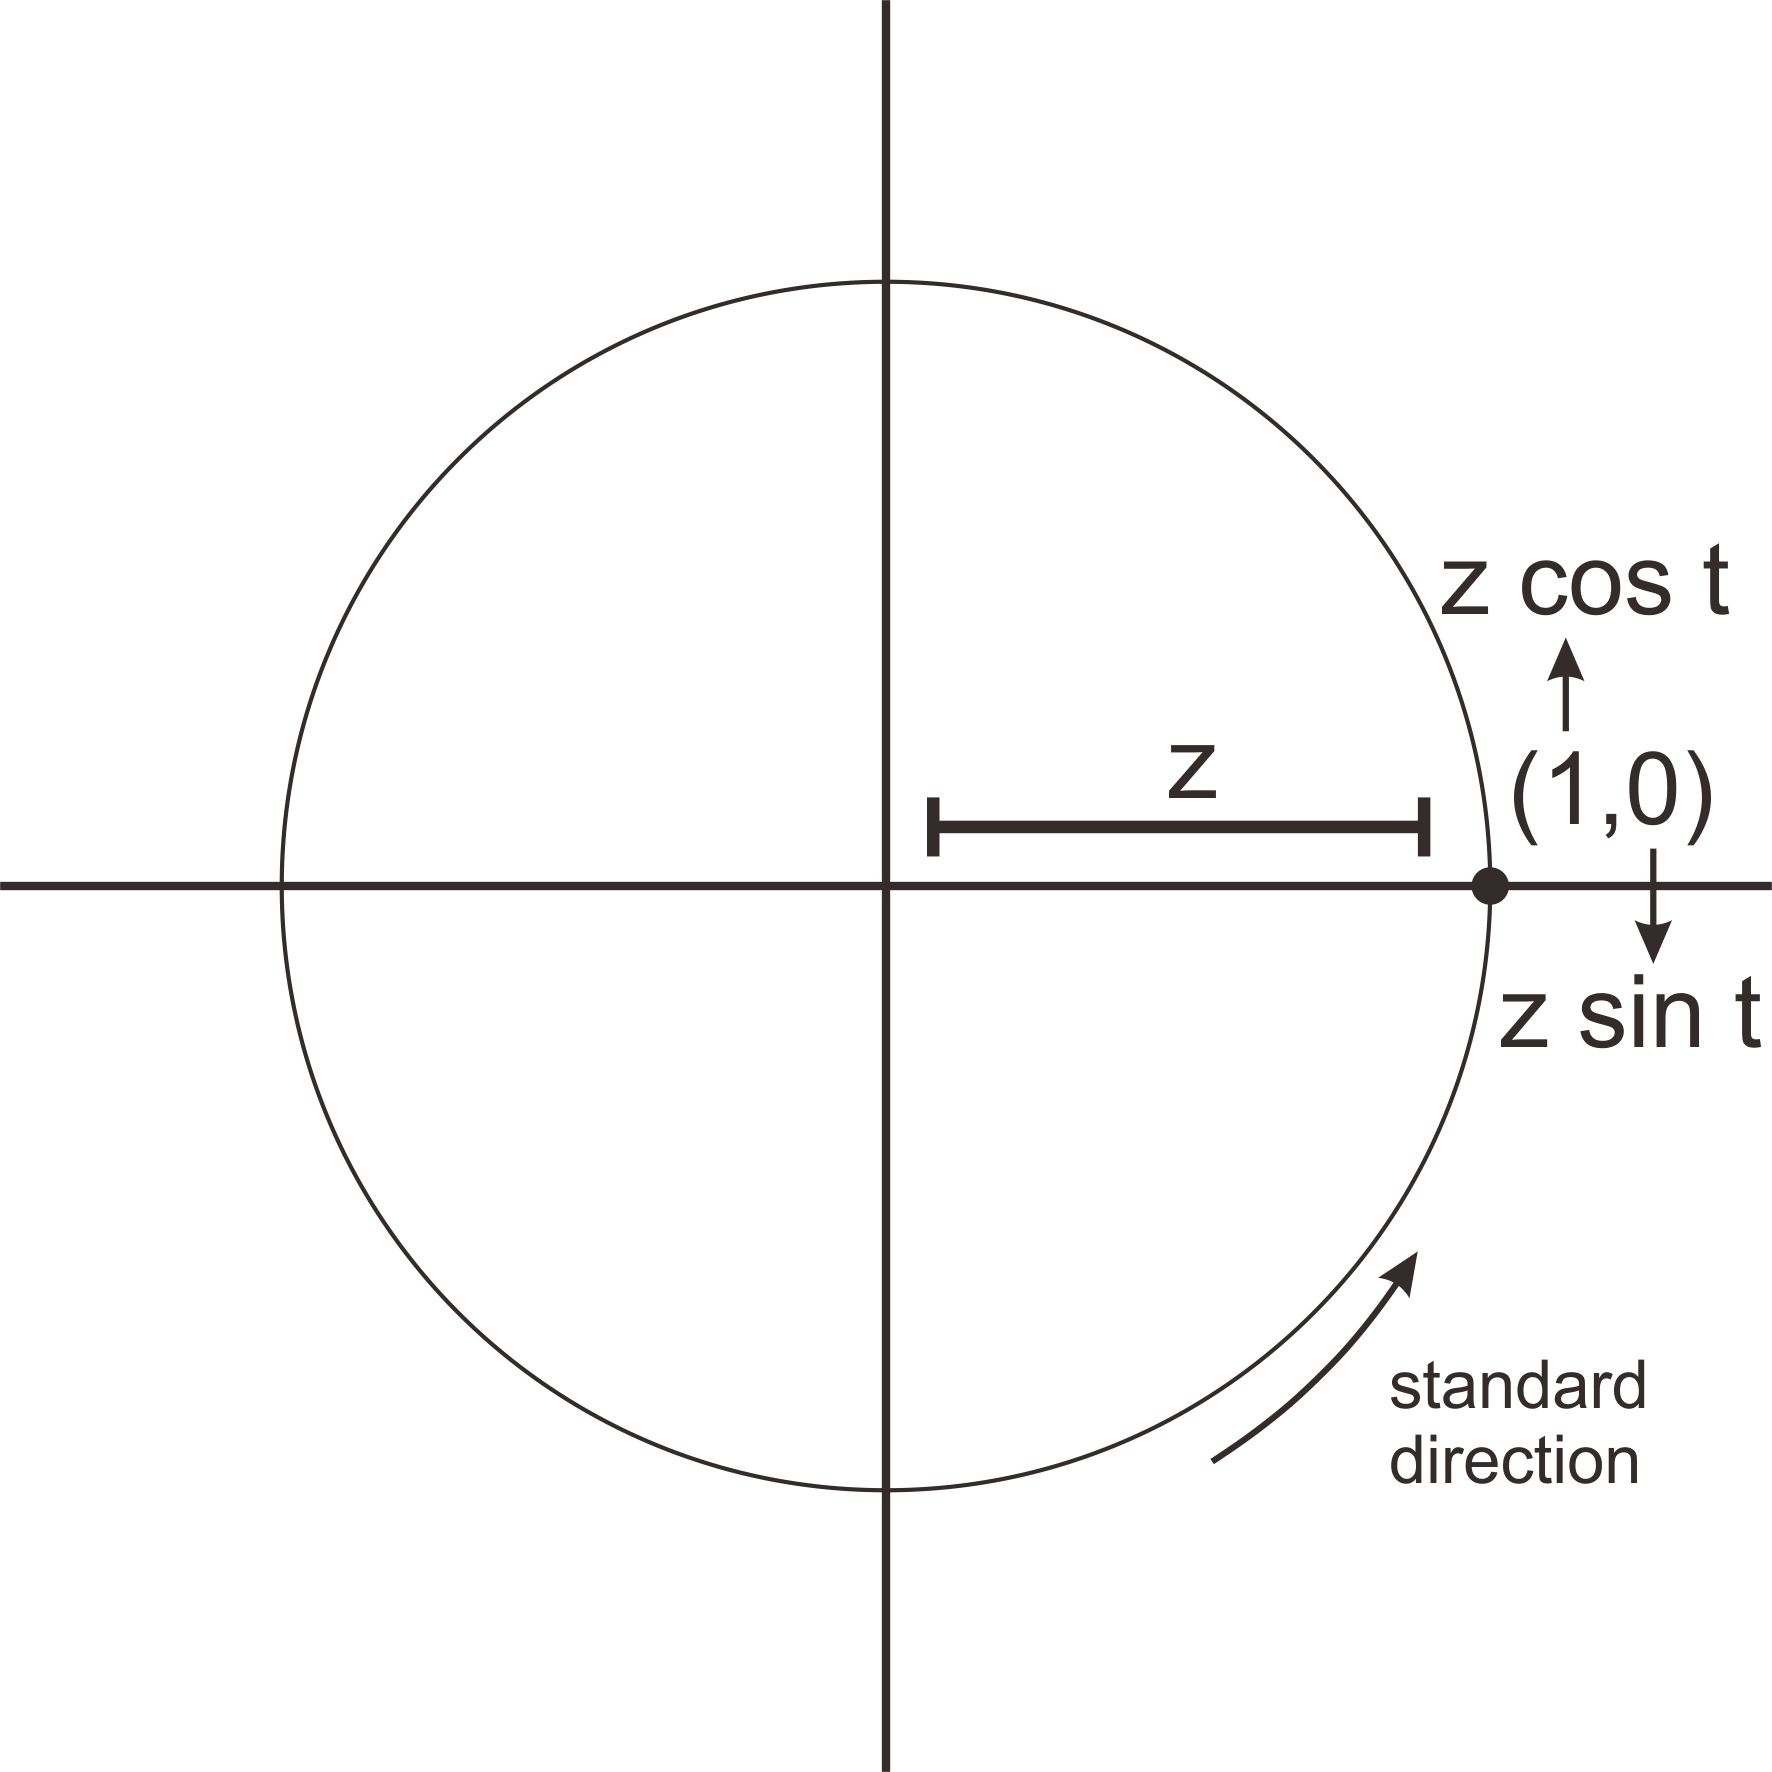
\includegraphics[width=0.37\linewidth]{picture/example1}
	\caption{Example 1}
	\label{fig:example1}
\end{figure}

Example 2:
\begin{equation}\nonumber
\begin{cases}
\text{border } a1(t=0,1) \{ x=t;y=0; \}\\
\text{border } a2(t-0,1) \{ x=1;y=t; \}
\end{cases}
\end{equation}

\begin{figure}[h!]
	\centering
	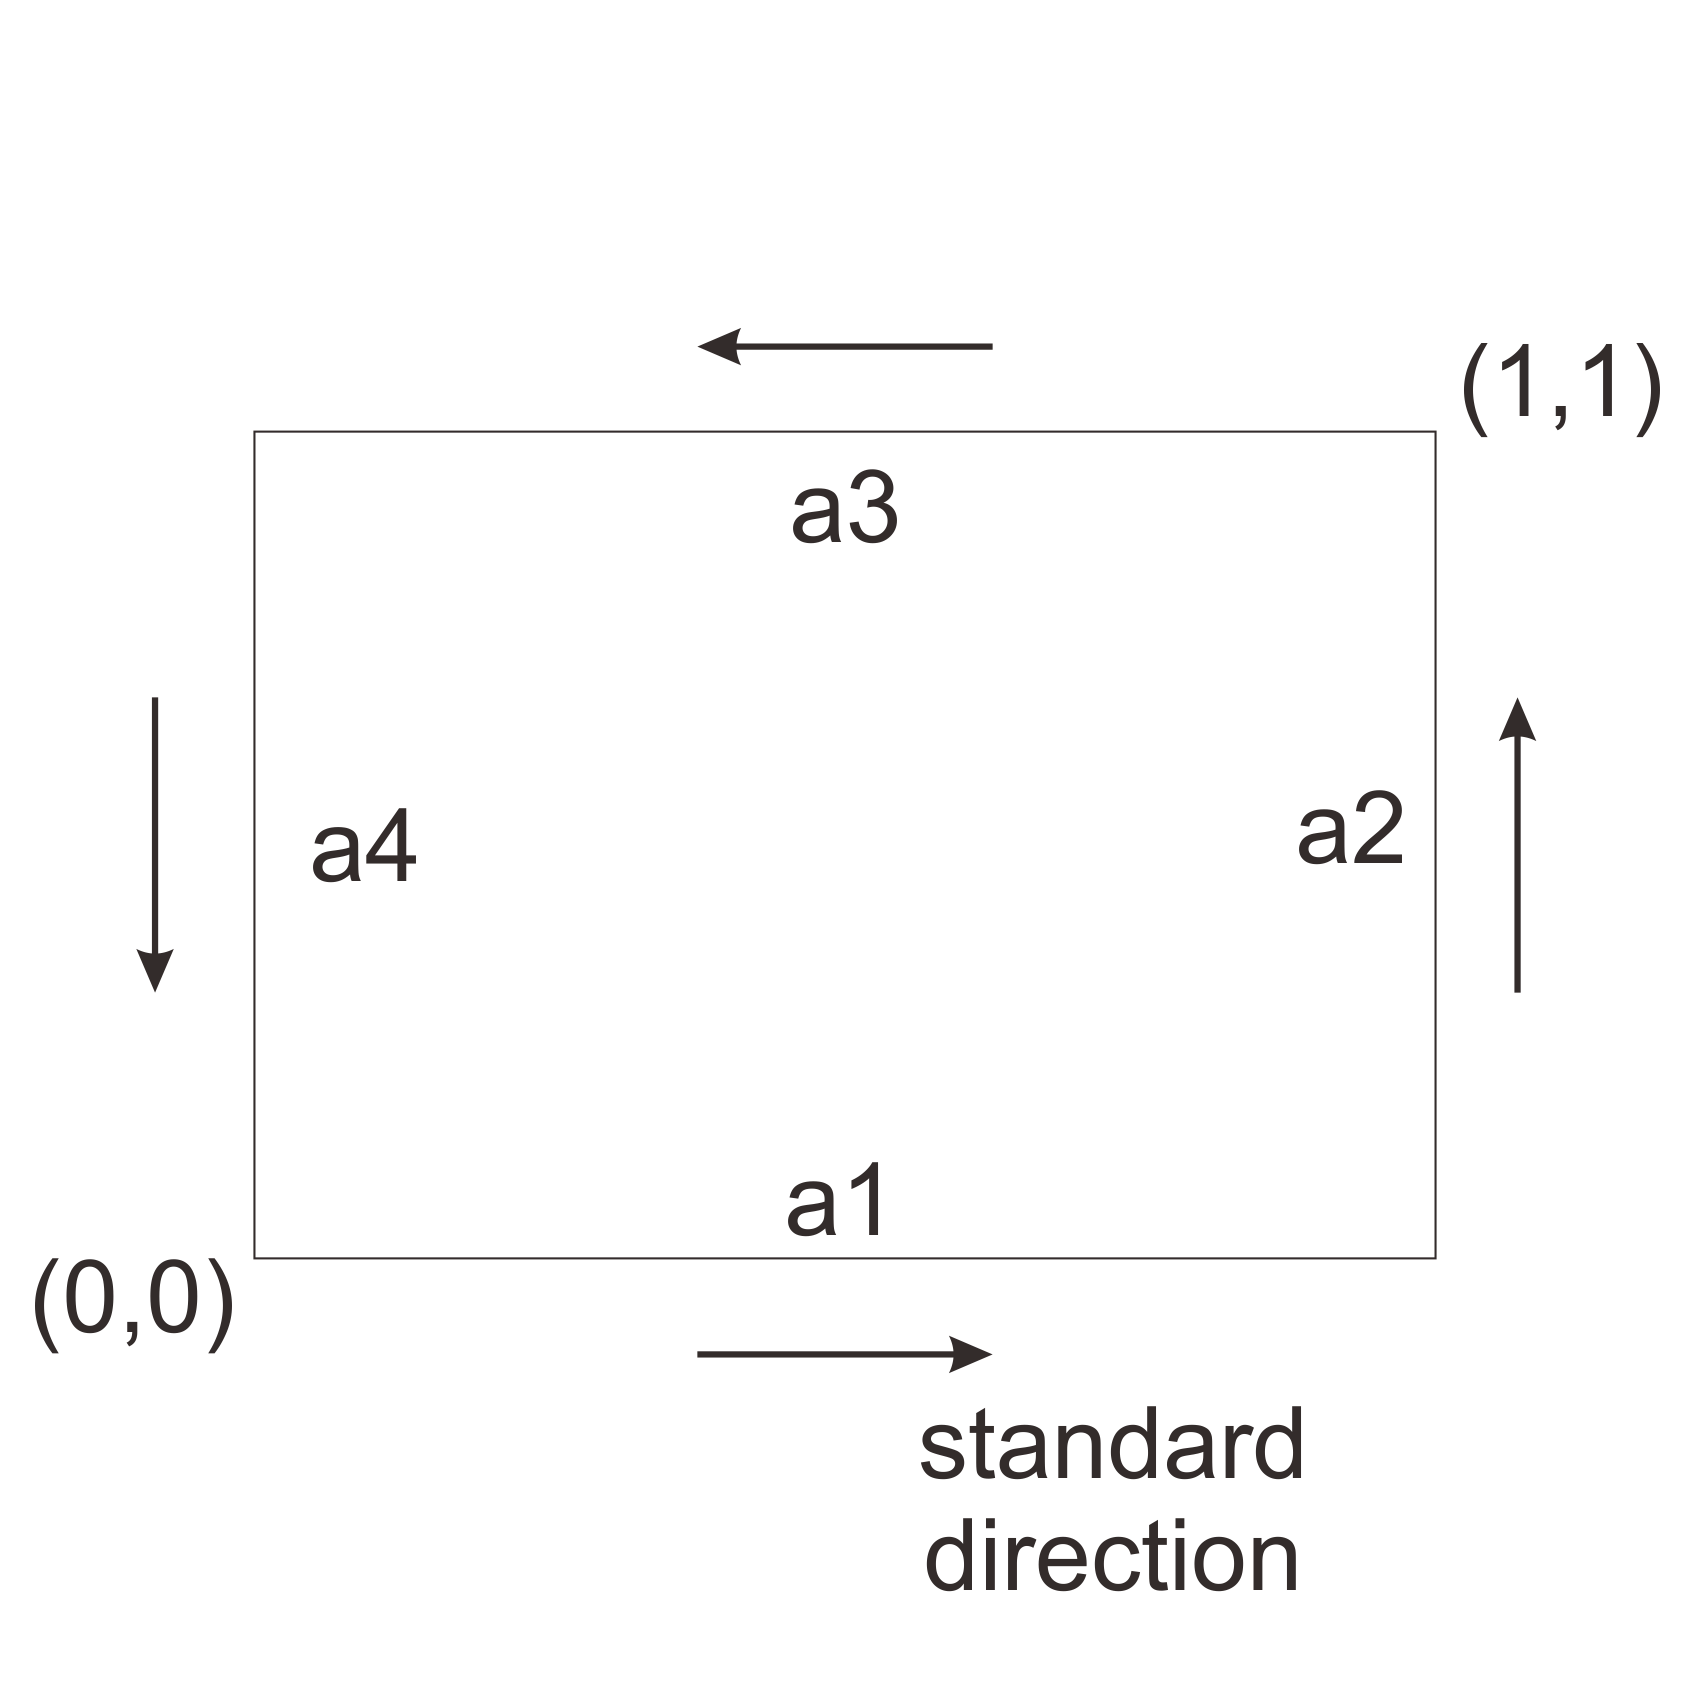
\includegraphics[width=0.37\linewidth]{picture/example2}
	\caption{Example 2}
	\label{fig:example2}
\end{figure}

\newpage
Here are image of how to choose the domain.
\begin{figure}[h!]
	\centering
	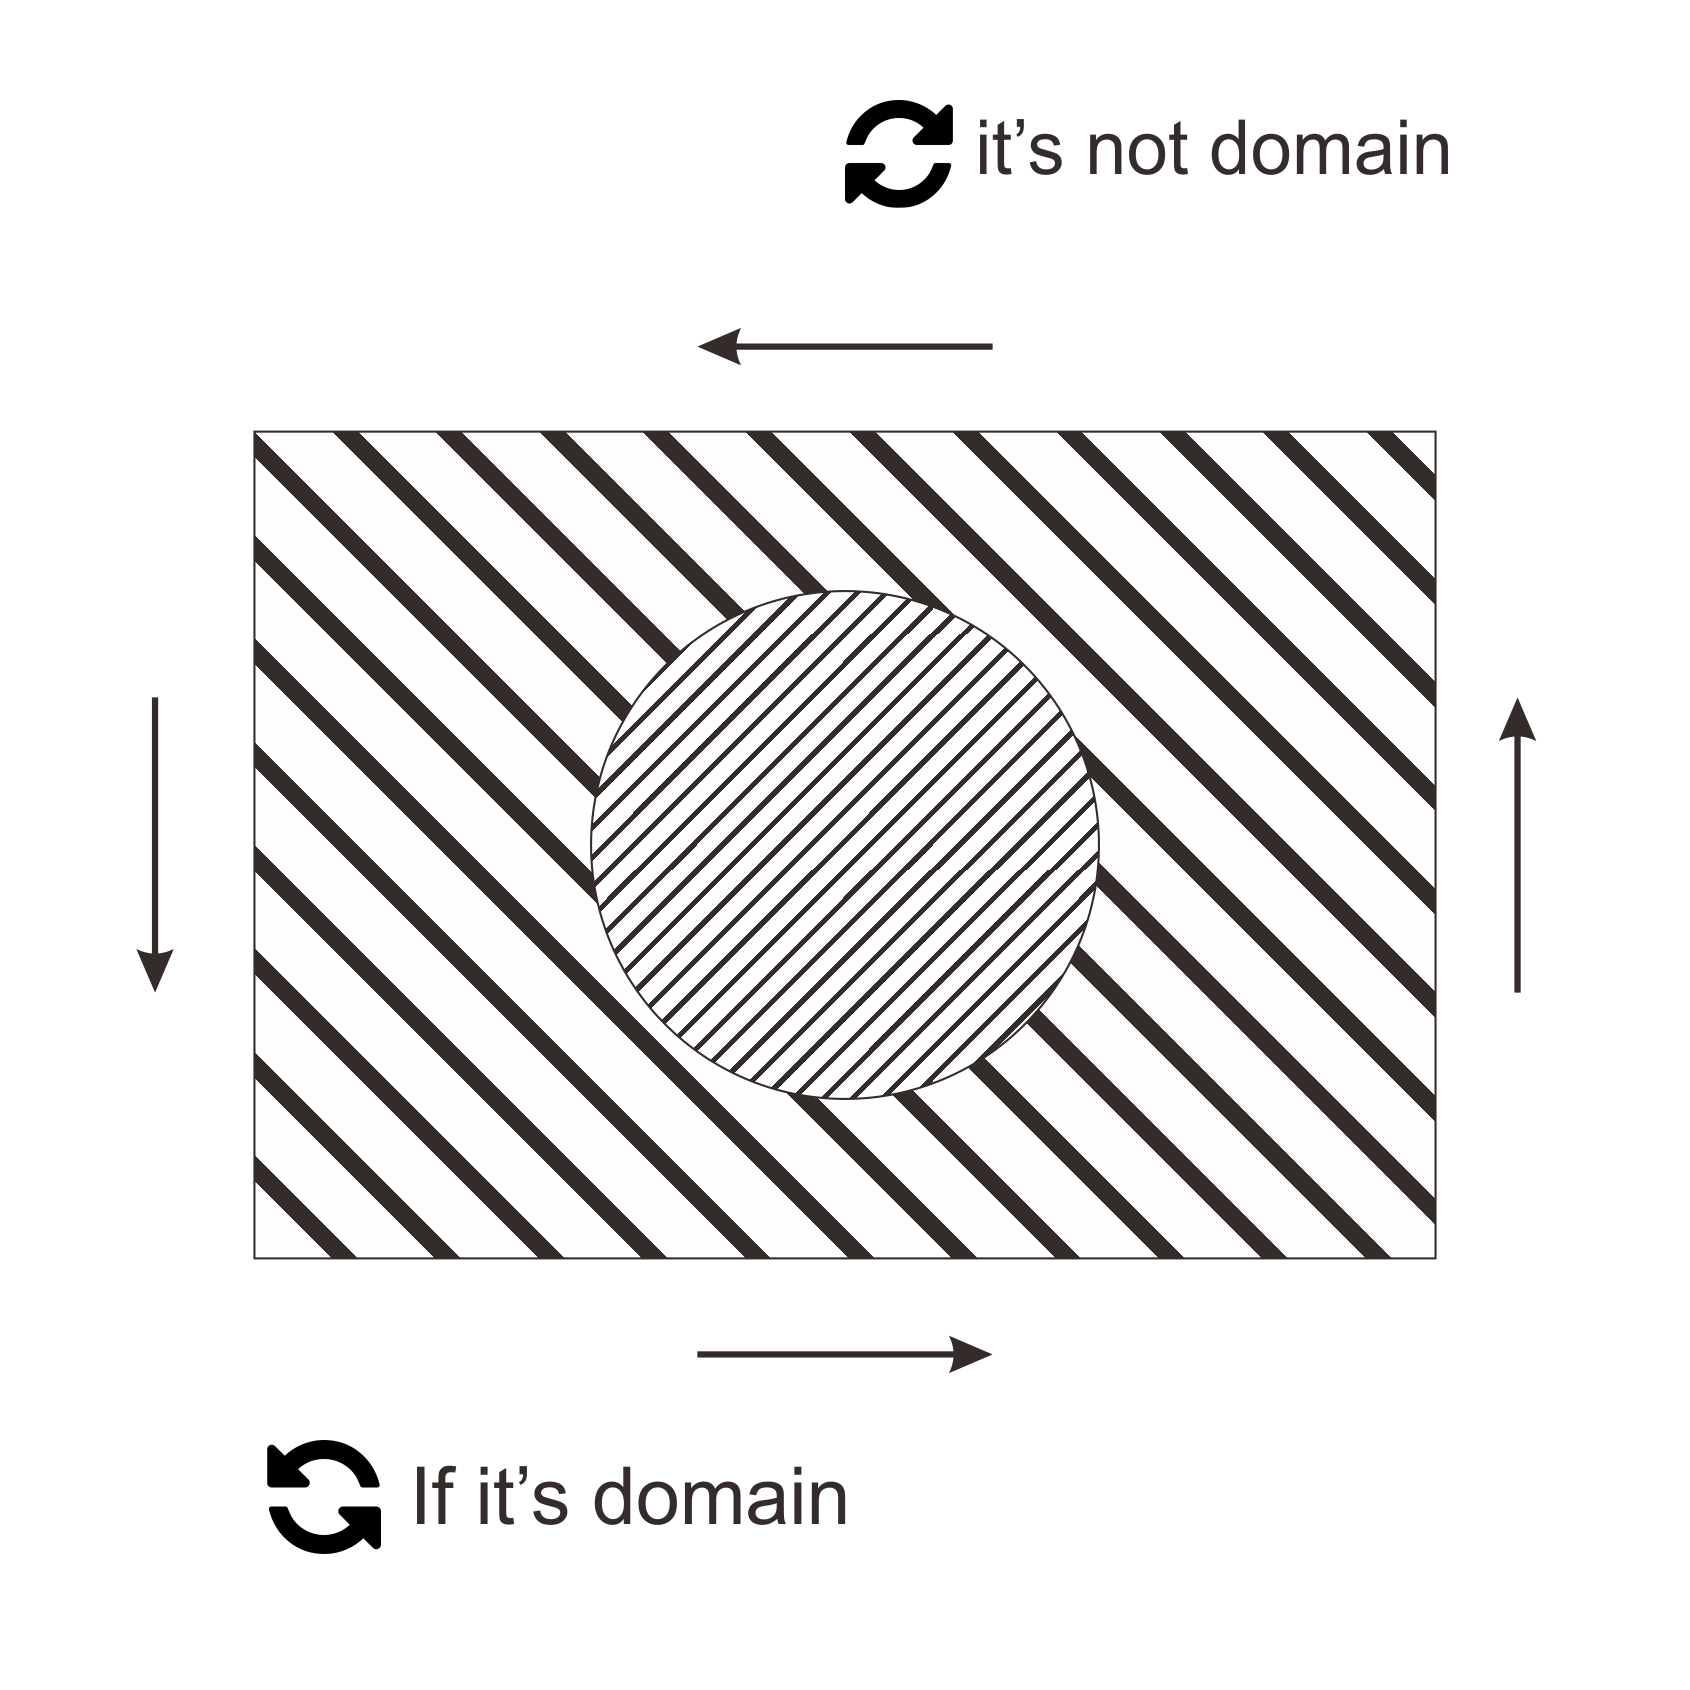
\includegraphics[width=0.5\linewidth]{picture/example2-2}
	\caption{Choose the domain}
	\label{fig:example2-2}
\end{figure}

From file : \textbf{membrane.edp}. Find $ \phi : \Omega \rightarrow \mathbb{R} $ such that
\begin{equation}\label{prob1}
\begin{cases}
-\bigtriangleup \phi = f (=1) & \text{in } \Omega \\
\phi = z (=x_{1}) & \text{on } \Gamma_{1} \\
\dfrac{\partial \phi}{\partial n} = 0 & \text{on } \Gamma_{2}
\end{cases}
\end{equation}
where $ f : \Omega \rightarrow \mathbb{R} $, given $ f(x)=1 $ and $ z : \Gamma_{1} \rightarrow \mathbb{R} $, given $ z(x)=x_{1} $. The equation (\ref{prob1}) is called \textbf{strong form}, because it contain second derivative.

\begin{figure}[h!]
	\centering
	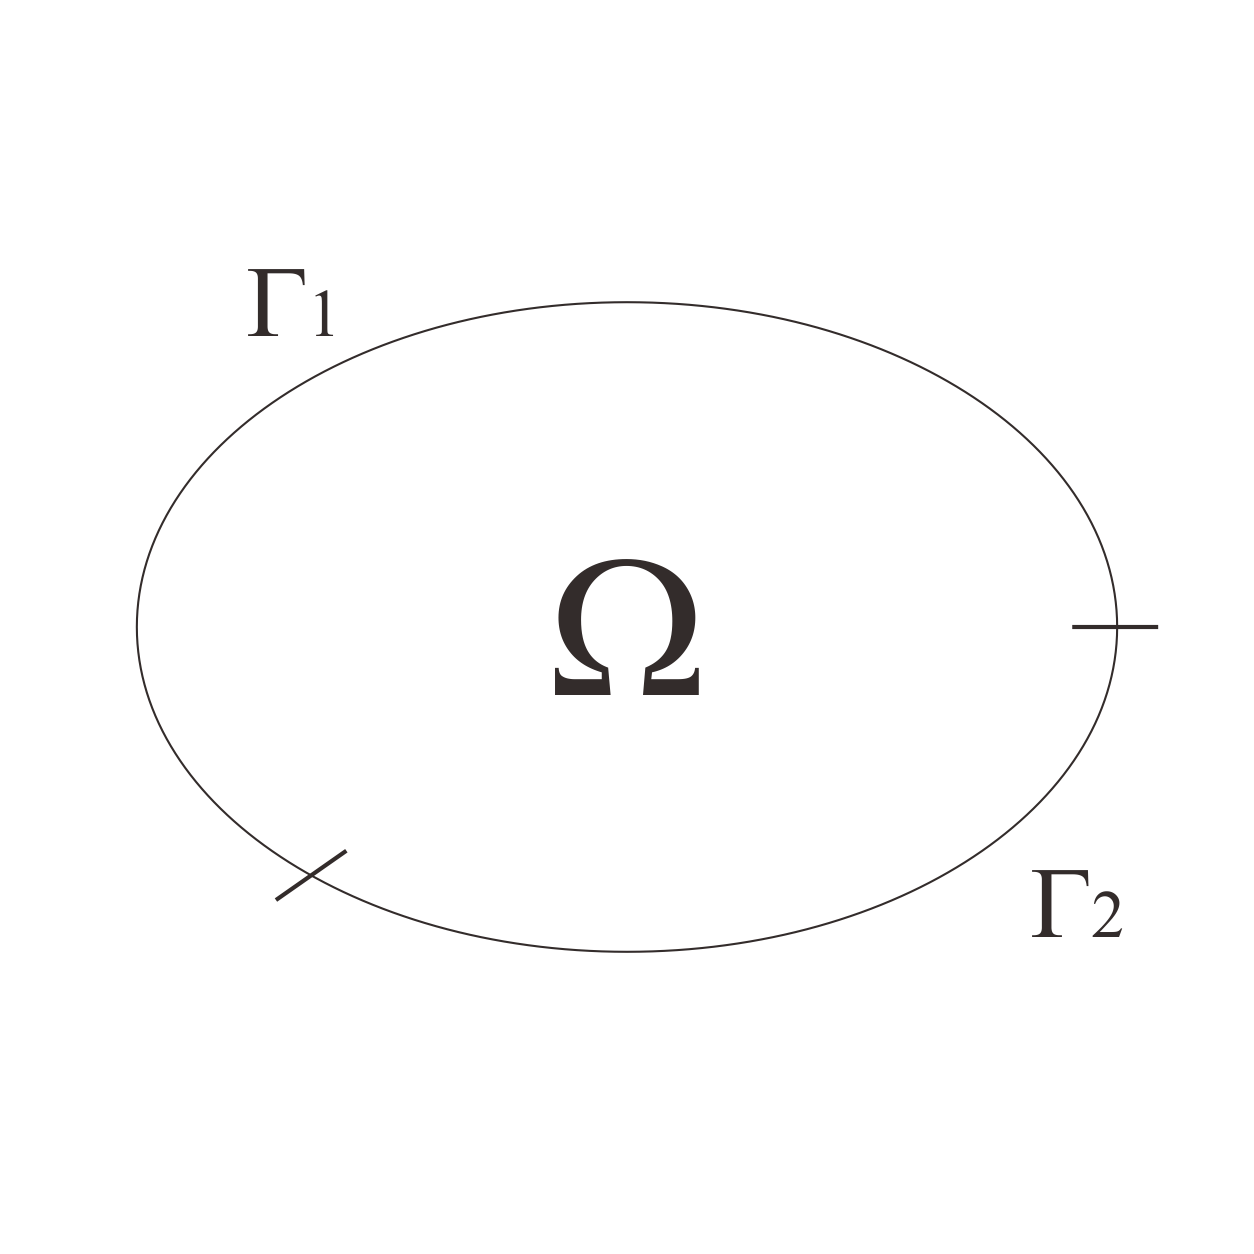
\includegraphics[width=0.4\linewidth]{picture/strongformdomain}
	\caption{}
	\label{fig:strongformdomain}
\end{figure}

From equation (\ref{prob1}) first line, we multiple it by smooth test function $ w $ and integrate over $ \Omega $ such that  $ \forall w (w|_{\Gamma_{1}}=0 ) $
\begin{equation*}\nonumber
\int_{\Omega} -\bigtriangleup \phi(x) w(x) \ dx = \int_{\Omega} f(x) w(x) \ dx
\end{equation*}
using integration by parts,
\begin{equation*}
-\int_{\partial\Omega} \dfrac{\partial \phi}{\partial n} (x) w(x) \ dx + \int_{\Omega} \bigtriangledown \phi(x) \cdot \bigtriangledown w(x) \ dx = \int_{\Omega} f(x) w(x) \ dx
 \end{equation*} 
 then we can devide the boundary such that
 \begin{equation*}
 -\int_{\Gamma_{1}} \dfrac{\partial \phi}{\partial n} (x) w(x) \ dx - \int_{\Gamma_{2}} \dfrac{\partial \phi}{\partial n} (x) w(x) \ dx + \int_{\Omega} \bigtriangledown \phi(x) \cdot \bigtriangledown w(x) \ dx = \int_{\Omega} f(x) w(x) \ dx
 \end{equation*} 
 Because on $ \Gamma_{1} $, smooth function $ w(x) $ value is equal to $ 0 $. And on $ \Gamma_{2} $ by equation (\ref{prob1}) line 3 we obtain that $ \dfrac{\partial \phi}{\partial n} (x) $ is equal to $ 0 $. Then, we conclude that
 \begin{equation}\label{prob1_weak}
 \int_{\Omega} \bigtriangledown \phi (x) \cdot \bigtriangledown w(x) \ dx - \int_{\Omega} f(x) w(x) \ dx =0
 \end{equation}
 is the \textbf{weak form}. Because it only contain first derivative.

\subsection{6 November 2017}

\subsubsection{Gauss-Green Formula}
In \textbf{2D Case}, we have $ f,g : \Omega \rightarrow \mathbb{R} $
\begin{equation}\label{GG2D}
\int_{\Omega} \dfrac{\partial f}{\partial x_{i}} (x) g(x) \ dx = \int_{\partial \Omega} f(x) g(x) n_{i} \ ds - \int_{\Omega} f(x) \dfrac{\partial g}{\partial x_{i}} (x) \ dx, \ (i=1,2)
\end{equation}

In \textbf{1D Case},
\begin{equation}\label{GG1D}
\int_{a}^{b} f(x) g(x) \ dx = [ f(x) g(x) ]_{x=a}^{b} - \int_{a}^{b} f(x) g'(x) \ dx
\end{equation}

\begin{eqnarray}\nonumber
\int_{\partial \Omega} f(x) g(x) n(x) \ dx & = & f(a)g(a)n(a) + f(b)g(b)n(b) \\ \nonumber
& = & [f(x)g(x)]_{x=a}^{b}
\end{eqnarray}


\subsubsection{Strong form}
Consider problem to find $ u : \Omega \rightarrow \mathbb{R} $ with \textbf{strong form} such as 
\begin{equation}\label{strong_form}
\begin{cases}
-\triangle u = f & \text{in } \Omega\\
u = g_{0} & \text{on } \Gamma_{0} \ \text{\textcolor{red}{Dirichlet (or essential) B.C.}} \\
\dfrac{\partial u }{\partial n} = g_{1} & \text{on} \Gamma_{1} \ \text{\textcolor{red}{Neumann (or natural) B.C. }}
\end{cases}
\end{equation}
where $ f : \Omega \rightarrow \mathbb{R} $ , $ g_{0} : \Gamma_{0} \rightarrow \mathbb{R} $ , and $ g_{1} : \Gamma_{1} \rightarrow \mathbb{R} $ is given.

\begin{figure}[h!]
	\centering
	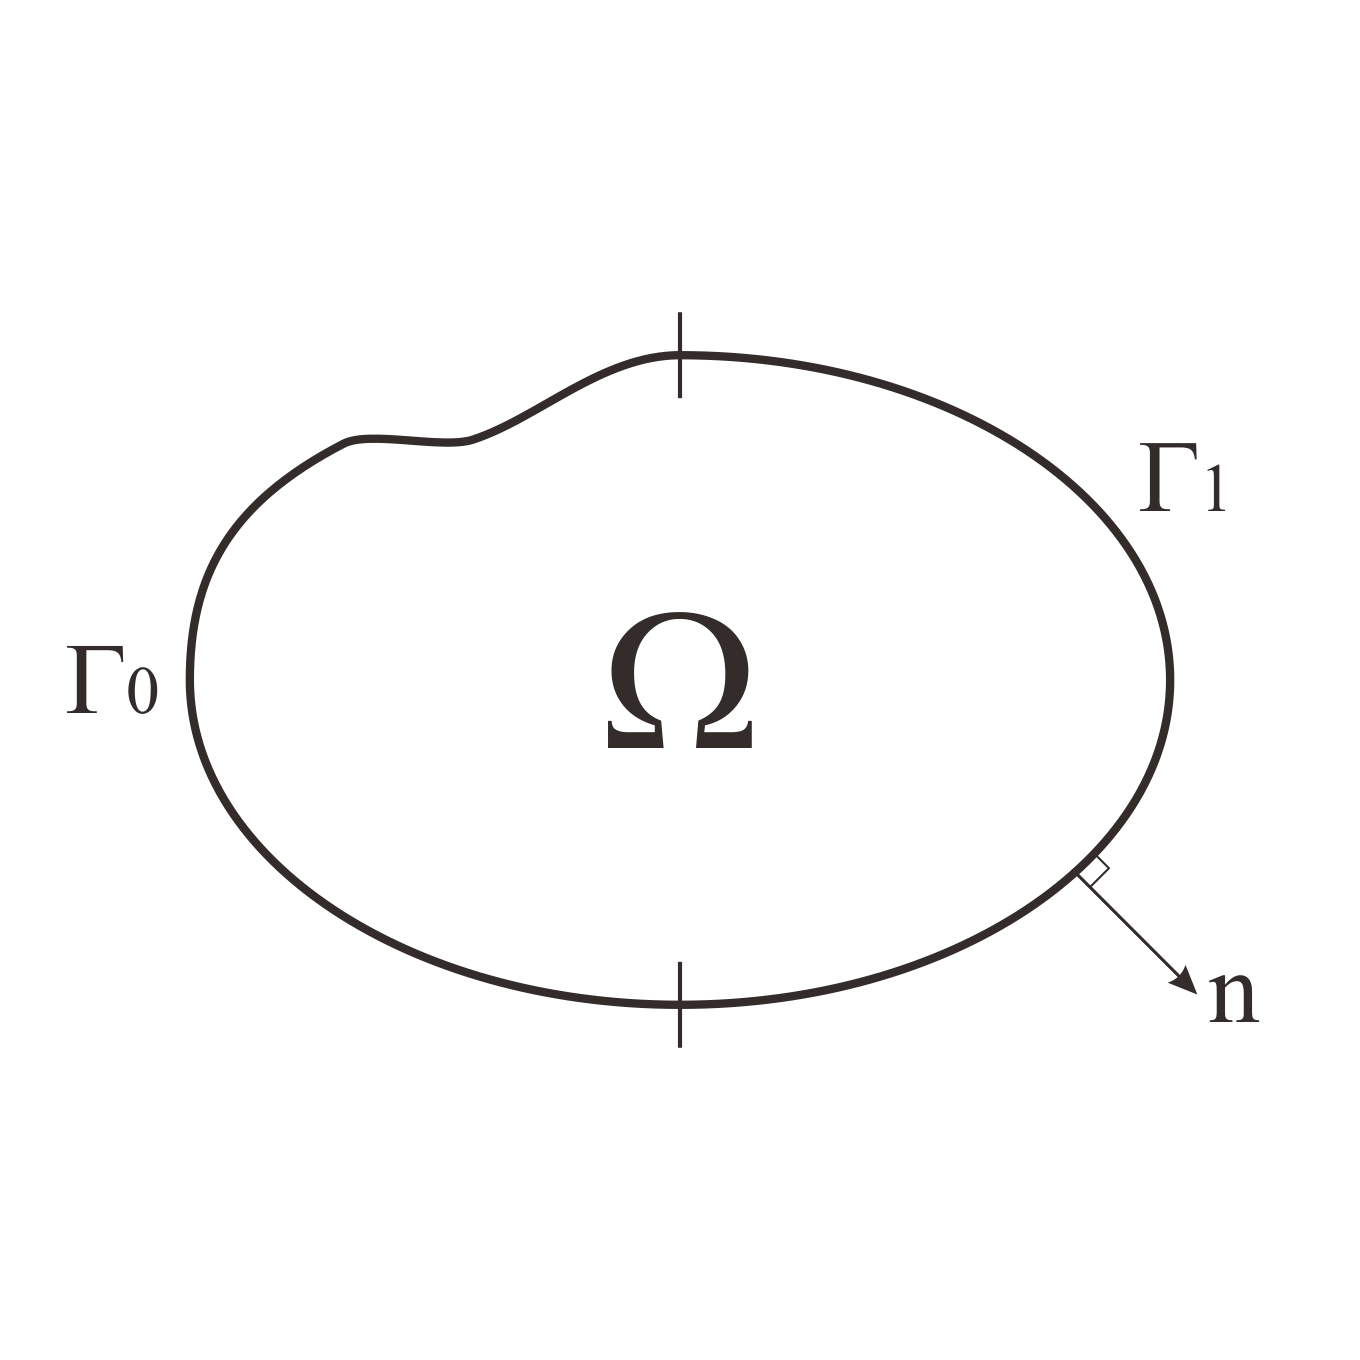
\includegraphics[width=0.5\linewidth]{picture/strongproblem}
	\caption{}
	\label{fig:strongproblem}
\end{figure}

\begin{eqnarray}\nonumber
\Omega &\subset &\mathbb{R}^2 \\ \nonumber
n &: \partial \Omega &\rightarrow \mathbb{R}^2 \\ \nonumber
&x &\mapsto n(x)
\end{eqnarray}

We have notation $ \bigtriangleup = \sum_{i=1}^{2} \dfrac{\partial^2}{\partial x_{1}^{2}} $ such that $ -\bigtriangleup u(x) = -\big( \dfrac{\partial^{2}}{\partial x_{1}^{2}} + \dfrac{\partial^{2}}{\partial x_{2}^{2}} u(x) \big) $. So we have
\begin{eqnarray}\nonumber
& -\bigtriangleup u(x) = f(x) \\ \nonumber
\leftrightarrow &  - \big( \dfrac{\partial^{2}}{\partial x_{1}^{2}} + \dfrac{\partial^{2}}{\partial x_{2}^{2}} \big) u(x) = f(x)
\end{eqnarray}

For all smooth test function $ v(x) $, where $ v|_{\Gamma_{0}}=0 $ and $ \int_{\Omega} \ dx $
\begin{eqnarray} \nonumber
 \int_\Omega (-\Delta u)(x) v(x) dx &=&\int_\Omega \Big(-\dfrac{\partial^2u}{\partial{x_1}^2} (x) v(x) -\dfrac{\partial^2u}{\partial{x_2}^2} (x) v(x) \Big) \ dx \\ \nonumber
&=& - \int_{\Omega} \dfrac{\partial^{2}u}{\partial x_{1}^{2}}  (x) v(x) \ dx - \int_{\Omega} \dfrac{\partial^{2} u}{\partial x_{2}^{2}} (x) v(x) \ dx\\ \nonumber
&=& - \Big( \int_{\partial \Omega} \dfrac{\partial u}{\partial x_{1}} (x) v(x) n_{i} \ ds - \int_{\Omega} \dfrac{\partial u}{\partial x_{1}} (x) \dfrac{\partial v}{\partial x_{1}} (x) \ dx \Big) \\ \nonumber
&& - \Big( \int_{\partial \Omega} \dfrac{\partial u}{\partial x_{2}} (x) v(x) n_{i} \ ds - \int_{\Omega} \dfrac{\partial u}{\partial x_{2}} (x) \dfrac{\partial v}{\partial x_{2}} (x) \ dx \Big) \\ \nonumber
&=& \Big( \int_{\Gamma_0} \dfrac{\partial u}{\partial x_{1}} (x) v(x) n_{i} + \dfrac{\partial u}{\partial x_{2}} (x) v(x) n_{i} \ ds \\ \nonumber
&& + \int_{\Gamma_1} \dfrac{\partial u}{\partial x_{1}} (x) v(x) n_{i} + \dfrac{\partial u}{\partial x_{2}} (x) v(x) n_{i} \ ds \Big) \\ \nonumber
&& + \int_{\Omega} \dfrac{\partial u}{\partial x_{1}} (x) \dfrac{\partial v}{\partial x_{1}} (x) + \dfrac{\partial u}{\partial x_{2}} (x) \dfrac{\partial v}{\partial x_{2}} (x) \ dx \\ \nonumber
&=& \int_{\Omega} \nabla u(x) \cdot \nabla v(x) \ dx - \int_{\Gamma_1} (\nabla u(x) \cdot n(x)) v(x) \ ds \\ \nonumber
&=& \int_{\Omega} \nabla u(x) \cdot \nabla v(x) \ dx - \int_{\Gamma_1} \dfrac{\partial u}{\partial n} (x) v(x) \ ds \\ \nonumber
&=& \int_{\Omega} \nabla u(x) \cdot \nabla v(x) \ dx - \int_{\Gamma_1} g_{1}(x) v(x) \ ds\\ \nonumber
&=& \int_{\Omega} f(x) v(x) \ dx
\end{eqnarray}
such that  
\begin{equation*}
\int_{\Omega} \nabla u \cdot \nabla v \ dx = \int_{\Omega} f v \ dx + \int_{\Gamma_1} g_{1} v \ ds
\end{equation*} 

\textbf{Note} : Reason why $ \dfrac{\partial u}{\partial n} (x) = (\bigtriangledown u ) \cdot n $
In 1D Case,
\begin{equation*}
u'(x) = \lim\limits_{h\rightarrow 0} \dfrac{u(x+h)-u(x)}{h}
\end{equation*}

\begin{figure}[h!]
	\centering
	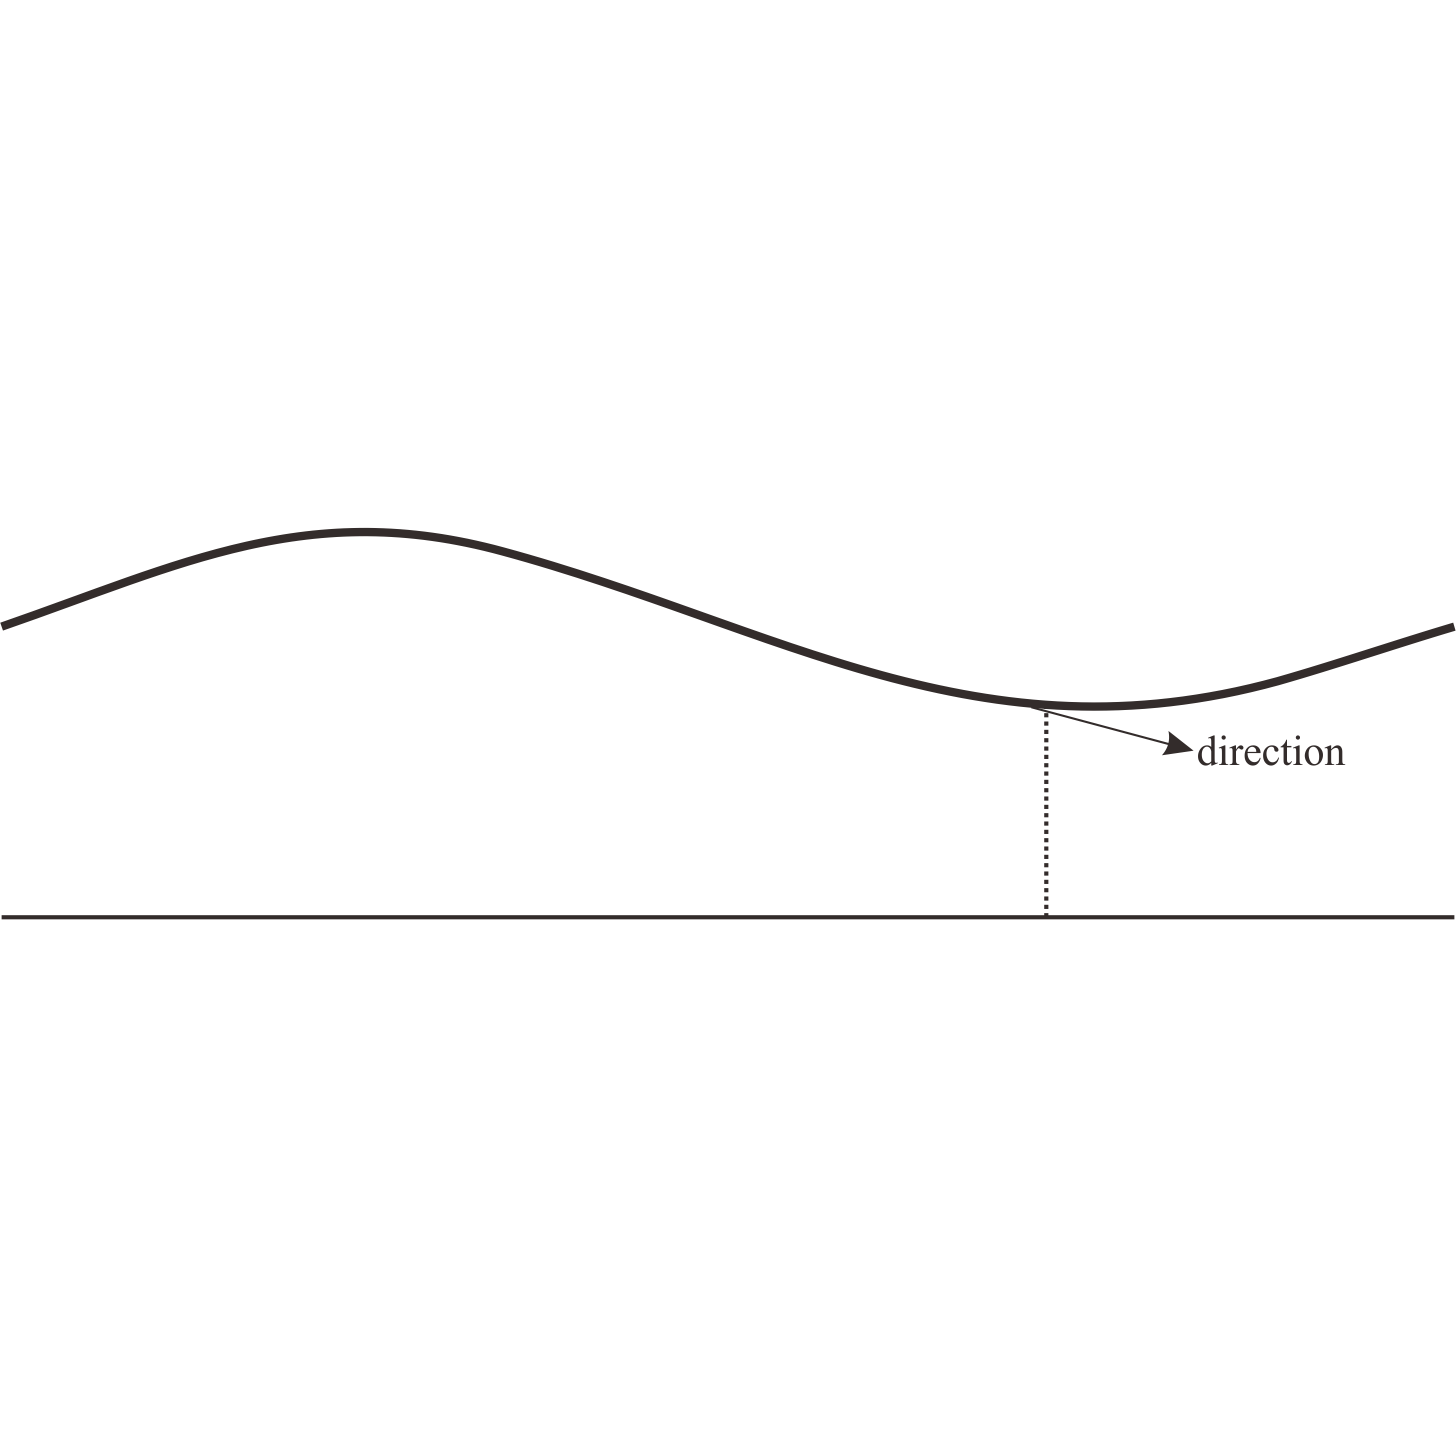
\includegraphics[width=0.5\linewidth]{picture/reasonIn1D}
	\caption{}
	\label{fig:reasonin1d}
\end{figure}


In 2D Case
\begin{eqnarray}\nonumber
\dfrac{\partial u}{\partial n}(x) &=& \lim\limits_{h \rightarrow 0} \dfrac{u(x+hn)-u(x)}{h} \\ \nonumber
&=& \lim\limits_{h \rightarrow 0} \dfrac{1}{h} \big[ u(x_{1}+hn_{1}, \ x_{2}+hn_{2}) - u(x_{1},x_{2}) \big] \\ \nonumber
&=& \lim\limits_{h \rightarrow 0} \dfrac{1}{h} \big[ u(x_{1}+hn_{1}, \ x_{2}+hn_{2}) - u(x_{1},x_{2}+hn_{2}) \\ \nonumber
& &+ u(x_{1},x_{2}+hn_{2}) - u(x_{1},x_{2})  \big] \\ \nonumber
&=& \lim\limits_{h \rightarrow 0} \dfrac{u(x_{1}+hn_{1}, \ x_{2}+hn_{2}) - u(x_{1},x_{2}+hn_{2})+ u(x_{1},x_{2}+hn_{2}) - u(x_{1},x_{2})}{hn_{1}} n_{1} \\ \nonumber
& & \lim\limits_{h \rightarrow 0} \dfrac{u(x_{1}+hn_{2}, \ x_{2}+hn_{2}) - u(x_{1},x_{2}+hn_{2})+ u(x_{1},x_{2}+hn_{2}) - u(x_{1},x_{2})}{hn_{2}} n_{2} \\ \nonumber
&=& \dfrac{\partial u}{\partial x_{1}} (x_{1},x_{2}) n_{1} + \dfrac{\partial u}{\partial x_{2}} (x_{1},x_{2})n_{2} \\ \nonumber
&=& (\nabla u) \cdot n
\end{eqnarray}

\subsubsection{Weak form}
We want to find $ u \in V(g_{0}) $ such that
\begin{equation*}
a(u,v) = l(v) , \ \forall v \in V
\end{equation*}
where 
\begin{equation*}
V(g_{0}) \equiv \{ v \in H^{1}(\Omega) ; \ v|_{\Gamma_{0}}=g_{0} \}, \ V \equiv V(0).
\end{equation*}
There are some notation we need to know beforehand,
\begin{equation*}
L^{2}(\Omega) \equiv \{ v : \Omega \rightarrow \mathbb{R} ; \int_{\Omega} v^{2}(x) \ dx < \infty \}.
\end{equation*}
For examples,
\begin{eqnarray}\nonumber
\Omega &=& (1,\infty) \\ \nonumber
f(x) &=& \dfrac{1}{x} \in L^{2}(1, \infty) ; \ \int_{1}^{\infty} f^{2}(x) \ dx = [ -x^{-1} ]^{\infty}_{1} =1 \\ \nonumber
f(x) &=& \dfrac{1}{\sqrt{x}} not \in L^{2}(1,\infty); \ \int_{1}^{\infty} \ dx = [log x]_{1}^{\infty} = \infty
\end{eqnarray}
Furthermore, $ L^2(\Omega) $ is a \textcolor{red}{Hilbert space} or complete space with inner product. 
\begin{equation*}
H^{1}(\Omega) \equiv \{ v \in L^2(\Omega); \ \dfrac{\partial v}{\partial x_{i}} \in L^2(\Omega), \ i=1,2. \}
\end{equation*}
Inner product is defined by
\[ (f,g) \equiv \int_{\Omega} f(x) g(x) dx. \]

Back to the problem, we have bilinear form $ a(u,v) $ and linear form $ l(v) $ as shown below.
\begin{eqnarray}\nonumber
a(u,v) &=&  \int_{\Omega} \nabla u \cdot \nabla v \ dx \\ \nonumber
l(v) &=& \int_{\Omega} f v \ dx + \int_{\Gamma_{1}} g_{1} v \ ds.
\end{eqnarray}
$ l(v) $ is called linear form, because it holds that
\[ l(\alpha v + \beta w) = \alpha l(v) + \beta l(w). \]
Then $ a(u,v) $ is called bilinear form because if $ u $ is fixed, them $ v $ is linear form respect to $ u $, and vice versa.

\subsubsection{Discretization}
We approach value of smooth function $ u(x) $ by piecewise linear function $ u_{h}(x) $ as
\[ u(x) ~ u_{h}(x) \equiv \sum_{i=1}^{Np} c_{i} \varphi_{i}(x) \]
where $ Np $ is total number of nodal points.

\vspace{4cm}

For case as shown by picture below,

\begin{figure}[h!]
	\centering
	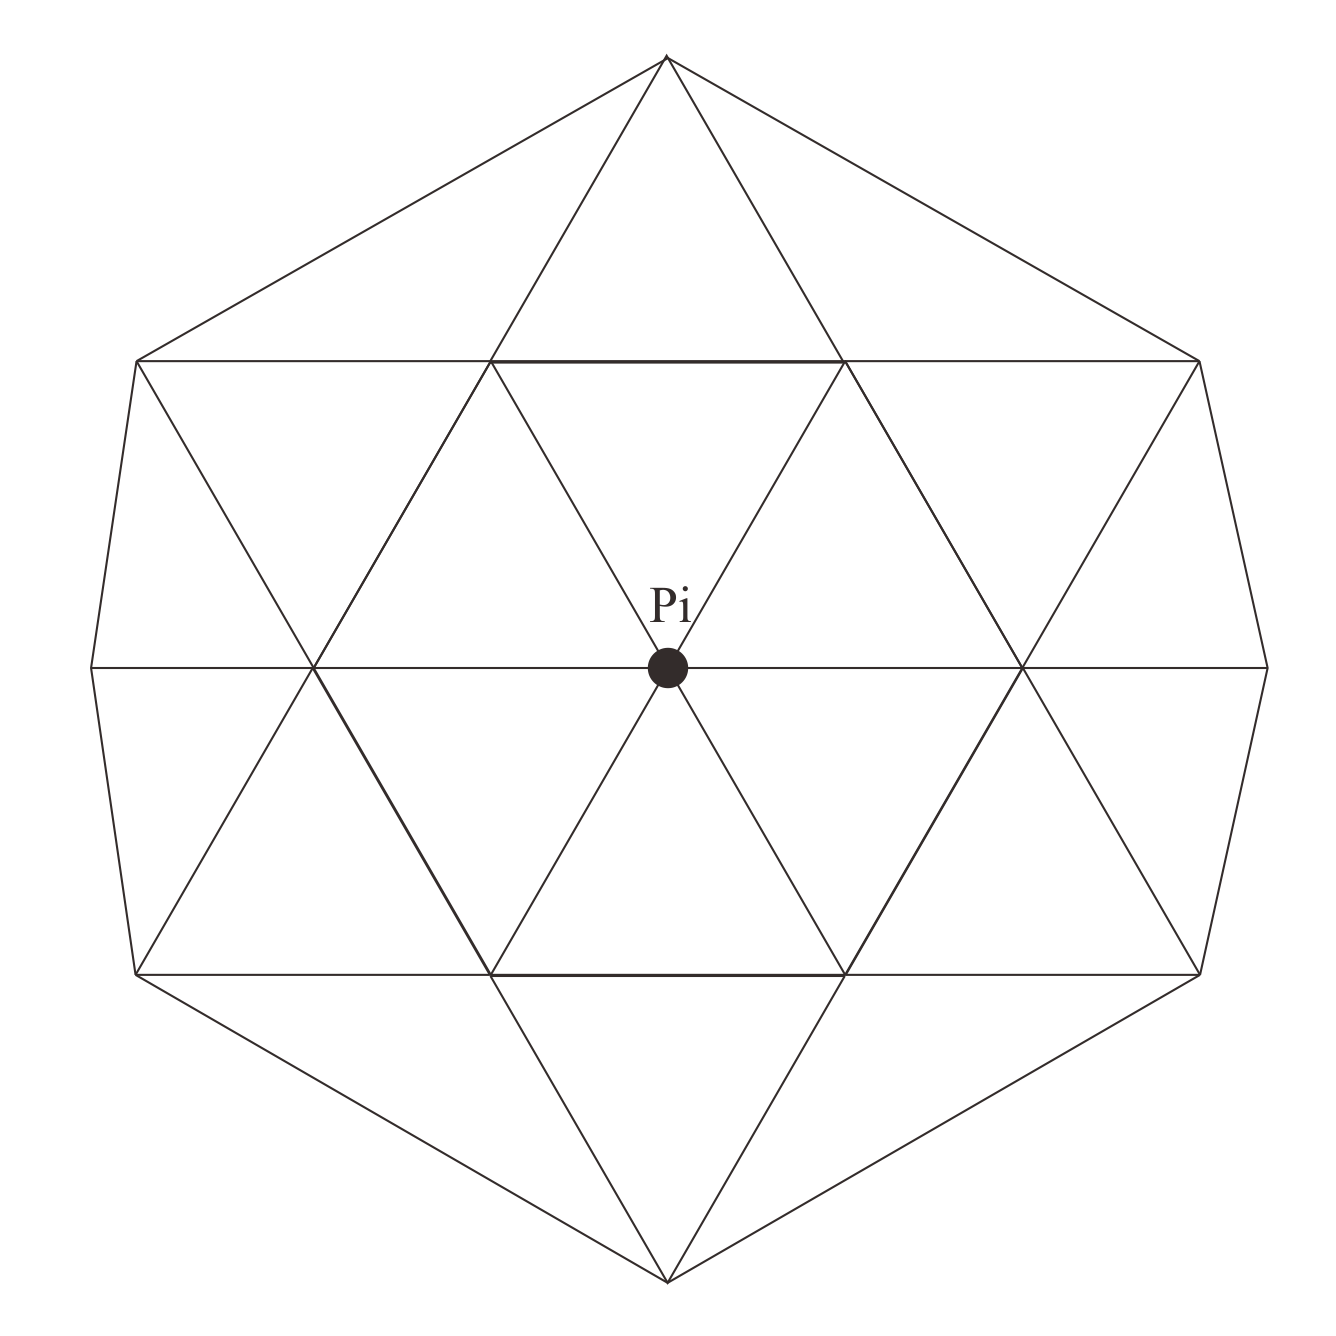
\includegraphics[width=0.5\linewidth]{picture/casepict}
	\caption{}
	\label{fig:casepict}
\end{figure}

we choose basis function
\begin{eqnarray}\nonumber
\varphi &:& \Omega \rightarrow \mathbb{R}\\ \nonumber
\varphi_{i} (P_{j}) &=& \begin{cases}
1 &, i=j, \\
0 &, i \neq j. 
\end{cases}
\end{eqnarray}
Then, in each triangle,
\[ \varphi_{i}(x) = \alpha_{0} + \alpha_{1}x_{1} + \alpha_{1}x_{2}. \]

\begin{figure}[h!]
	\centering
	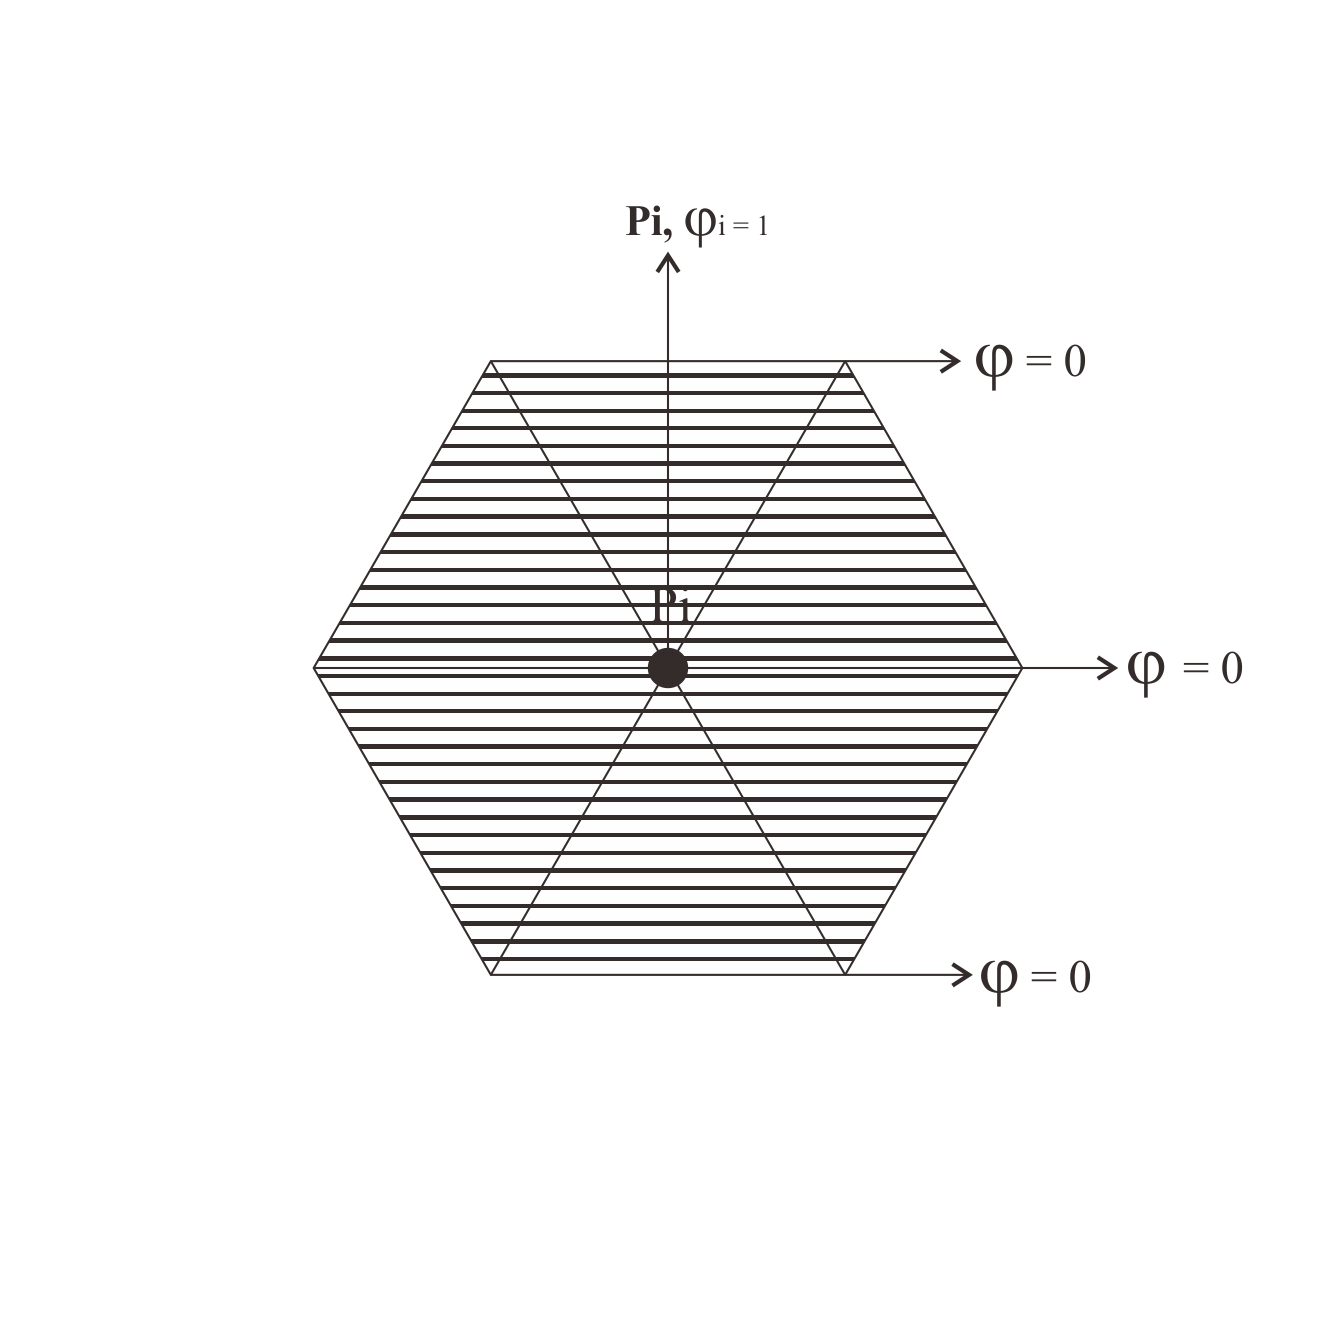
\includegraphics[width=0.4\linewidth]{picture/eachtriangle}
	\caption{}
	\label{fig:eachtriangle}
\end{figure}


Then, the problem becomes we want to find $ u_{h} \in V_{h}(g_{0}) $ such that
\[ a(u_{h}, v_{h}) = l(v_{h}), \ \forall v_{h} \in V_{h} \]
where
\[ V_{h}(g_{0}) \equiv \{ v_{h} \in V(g_{0}); \ v_{h}(x) = \sum_{i=1}^{Np} c_{i} \varphi_{i}(x), \ c_{i} \in \mathbb{R}, \ \varphi_{i} \text{ is basis function} \} , \ V_{h} \equiv V_{h}(0). \]

\subsubsection{Problem}
For simplicity, assume $ \Omega = (0,1)^2 $ and $ g_{0} $ = 0. We want to find $ u \in V \equiv H_{0}^{1}(\Omega) $ or Sobolev space where the boundary is $ 0 $. $ \{ P_{i} \}_{i=1}^{Np} $ is set of nodal points. For example,

\begin{figure}[h!]
	\centering
	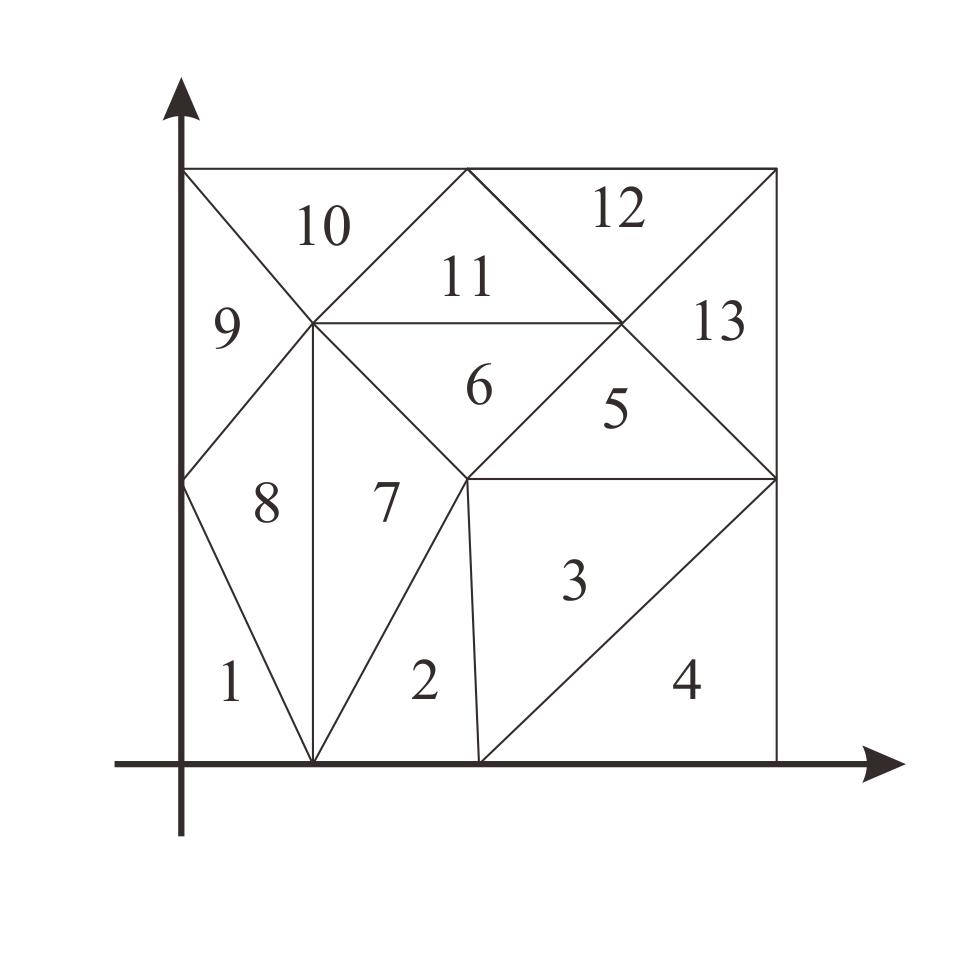
\includegraphics[width=0.5\linewidth]{picture/problem}
	\caption{}
	\label{fig:problem}
\end{figure}
with nodal point $ Np =11 $ and elements $ Ne =13 $.  The domain $ \tau_{h}= \{K_{k}\}_{k=1}^{13} $ or devided into $ 13 $ triangle area with point $ \{P_{i}\}_{i=1}^{11} $. Using file \textcolor{blue}{Square.edp} and \textcolor{blue}{mesh.msh}, we can read the mesh grid as shown below.

\begin{figure}[h!]
	\centering
	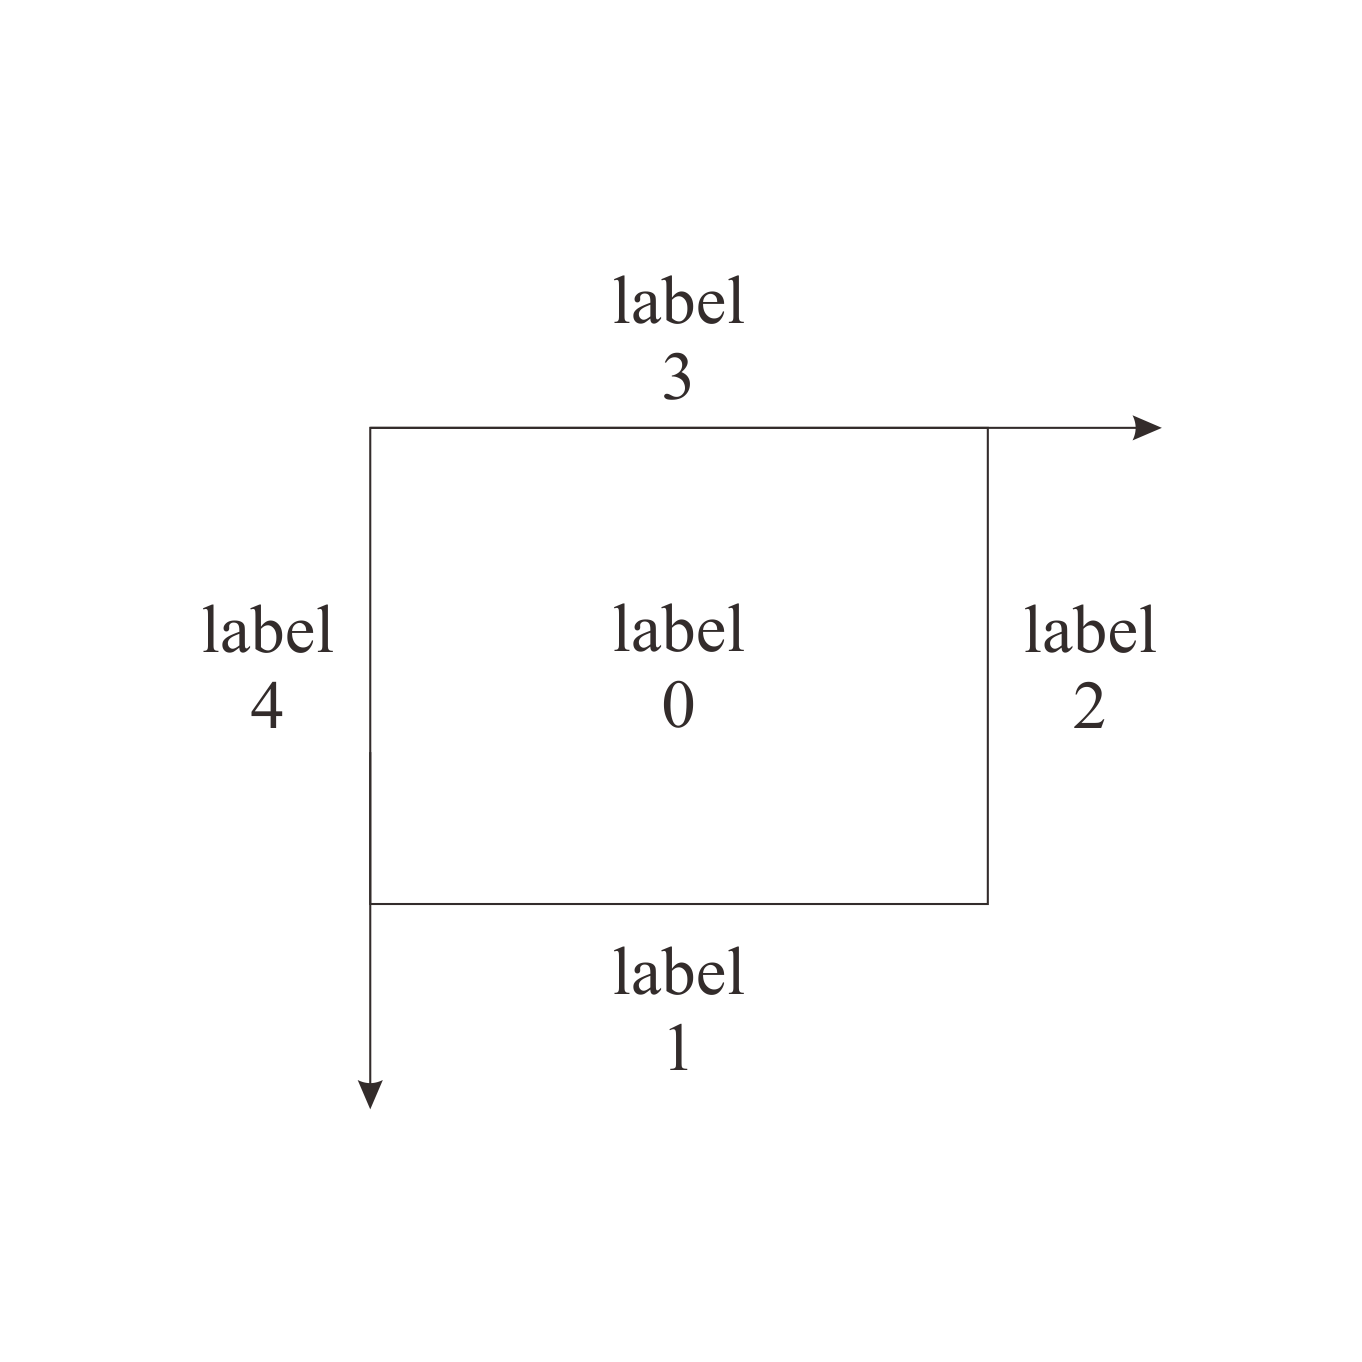
\includegraphics[width=0.53\linewidth]{picture/labelPict}
	\caption{}
	\label{fig:labelpict}
\end{figure}
\begin{figure}[h!]
	\centering
	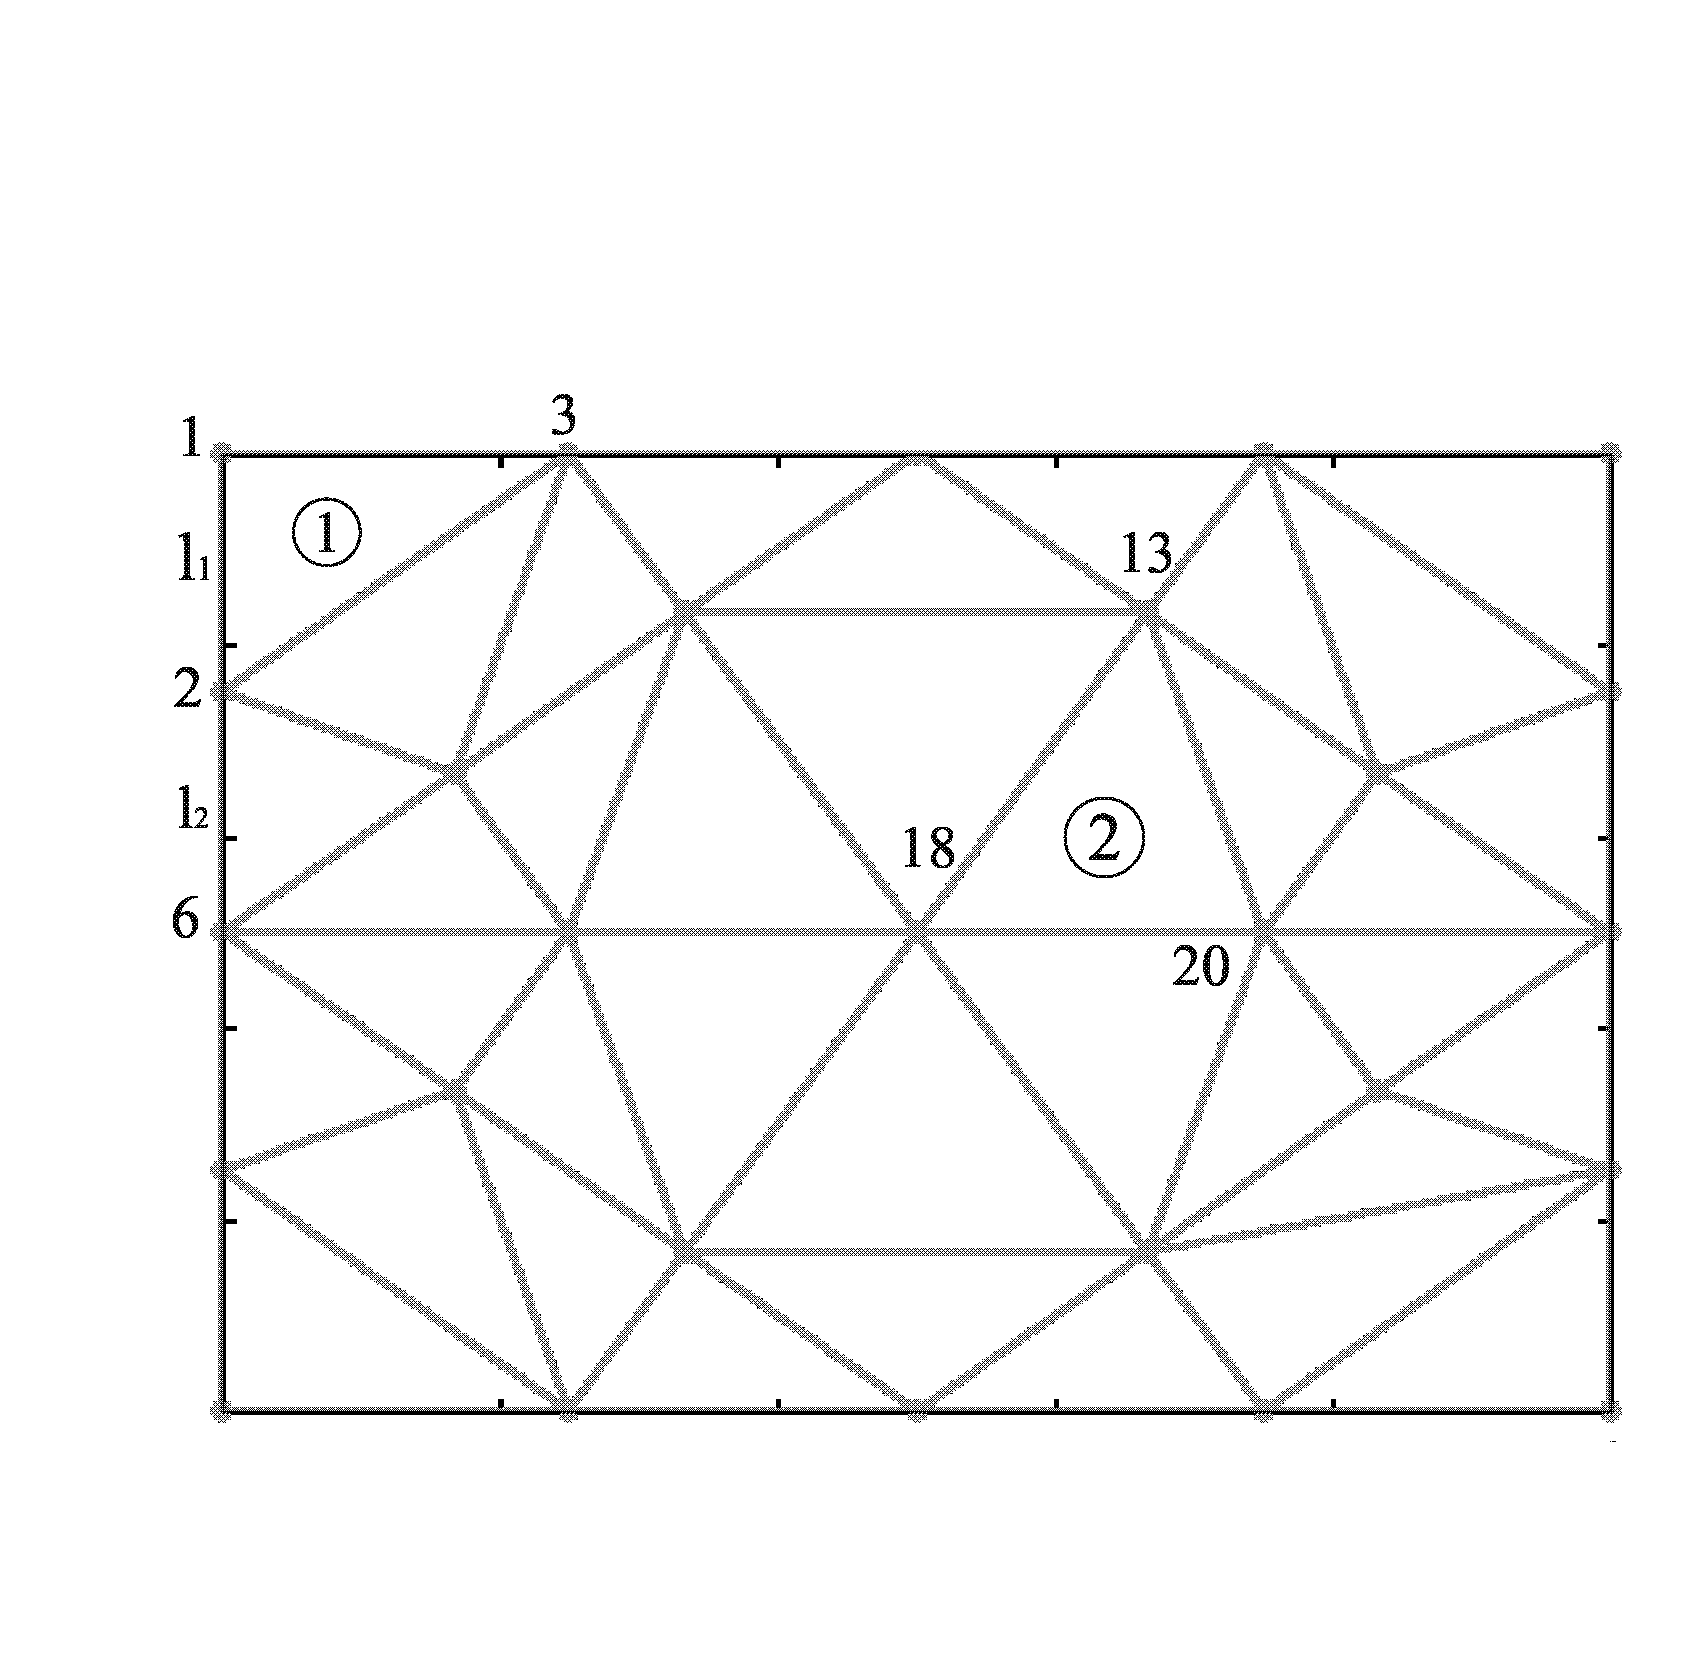
\includegraphics[width=0.7\linewidth]{picture/trianglePict}
	\caption{}
	\label{fig:trianglepict}
\end{figure}


Result : \textcolor{blue}{Master/Seminar/1.Read\_mesh/test.c}

\subsection{13 November 2017 (LINEAR ELASTICITY)}

\subsubsection{Basic Equations}
Let $ \Omega $ be a non-deformed reference configulation of an elastic body in 3d. We assume $ \Omega $ is a bounded Lipschitz domain in $ \mathbb{R}^{3} $. The position vector in $ \overline{\Omega} $ is denoted by $ x = (x_{1},x_{2},x_{3})^{T} \in \overline{\Omega} \subset \mathbb{R} $. For other notation, we use $ \partial_{j} := \dfrac{\partial}{\partial x_{j}} $, $ \bigtriangledown = (\partial_{1}, \partial_{2}, \partial_{3})^{T} $, $ \bigtriangledown^{T} u = (\partial_{j}u_{i}) \in \mathbb{R}^{3\times3} $, and $ \bigtriangledown u^{T} = (\bigtriangledown^{T} u)^{T}$ for $ u(x) \in \mathbb{R}^{3} $.

\subsection{20 November 2017}

\subsection{4 December 2017}

\subsubsection{Continuous (Partial Differential Equation)}
To show that there is exist unique solution $ u $, we can use the Remark below. 
\begin{remark}
	$ \exists ! u = \underset{v \in V(g)}{argmin} \ (\dfrac{1}{2} a(v,v)-l(v)) = \underset{w \in V(g)}{argmin} \ J(w)$
\end{remark}

minimizer or $ argmin $ is value of $ x $ where the function $ f(x) $ is minimum. For example, for function $ f(x)=1+x^2 $, $ \underset{x \in \mathbb{R}}{min} f(x) = f(0) =1 $. Then, the minimizer, $ \underset{x \in \mathbb{R}}{argmin} f(x) = 0 $.

Using this Remark, the Proposition below is given with proof.
\begin{prop}
	For $ J(v) := \dfrac{1}{2} a(v,v) -l (v) $,
	$ u = \underset{v \in V(g)}{argmin} \ J(v) \iff a(u,v)=l(v) $
\end{prop}

\textbf{Proof:}\\
$ (\Rightarrow) $ if $ u = argmin \ J $ then $ u+tv \in V(g) , \ \forall t \in \mathbb{R}, \forall v \in V = H_{0}^{1} (\Omega) $. Since it is on boundary $ \Gamma $, then $ g=u=u+tv $.
\begin{eqnarray}\nonumber
J(u) &\leq J(w) &, \forall w \in V(g), \ w=u+tv \in V(g)\\ \nonumber
J(u) &\leq J(u+tv) &, \forall t \in \mathbb{R}, \ \forall v \in V
\end{eqnarray}
Then
\begin{eqnarray}\nonumber
J(u+tv) &=& \dfrac{1}{2} a(u+tv,u+tv)-l(u+tv)\\ \nonumber
&=& \dfrac{1}{2} a(u,u) + t a(u,v) + \dfrac{t^2}{2} a (v,v) - l(u) - t l(v)\\ \nonumber
&=& \dfrac{t^2}{2} a (v,v) + t (a(u,v) - l(v)) + J(u)\\ \nonumber
&=:& \varphi(t)
\end{eqnarray}
Because $ \varphi(t) $ is in quadratic form, then its minimum obtained at $ t=0 $. So that $ \varphi =0 $ such that $ a(u,v) - l(v) =0 $.\\
$ (\Leftarrow) $ $ \forall t \in \mathbb{R}, \forall v \in V $ we have
\begin{equation}\nonumber
J(u,tv) = J(u) + \dfrac{t^2}{2} a(v,v) \geq J(u).
\end{equation}
$ \forall w \in V(g) $, we set $ v := w -u \in V , \ t:=1 , \ w=u+tv $
\begin{equation}\nonumber
J(w) = J(u+tv) \geq J(u)
\end{equation}

\subsubsection{Discrete (Finite Element Method)}
Here introduced some notation,
\begin{eqnarray}\nonumber
X_{h} &\subset & X \text{ (usually dim } X_{h} < \infty \text{)} \\ \nonumber
V_{h} & = & X_{h} \cap V\\ \nonumber
g_{h} & \in & X_{h} \text{(approximation of } g \text{)} \\ \nonumber
V_{h}(g_{h}) & = & \{ v_{h} \in X_{h} ; v_{h}-g_{h} \in V_{h} \}.
\end{eqnarray}
Then the weak form is approximated with
\begin{equation} \nonumber
\begin{cases}
a(u_{h}, v_{h}) &= l(v_{h}), \ \forall v_{h} \in V_{h} \\
u_{h} &\in V_{h}(g_{h})
\end{cases}
\iff u_{h} = \underset{w_{h} \in V_{h}(g_{h})}{argmin}J(w_{h})
\end{equation}

Using Finite Element Method,
\begin{eqnarray}\nonumber
X_{h} &=& \{ v_{h} \in C^{0}(\overline{\Omega}) ; \ {v_{h}|}_{K} \text{ is linear} \} \\ \nonumber
V_{h} &=& X_{h} \cap H_{0}^{1}(\Omega),
\end{eqnarray}
or we could write
\begin{eqnarray} \nonumber
X_h &=& \langle \varphi_1, \dots  , \varphi_{Np} \rangle\\ \nonumber
&=& \{\sum_{i=1}^{Np} c_i\varphi_i \ ; \ c_i \in \mathbb{R} \}
\end{eqnarray}
where $ \{\varphi_i\}^{Np}_{i=1} \text{ become a basis of the vector space } X_h $. For nodal points $ \{P_{i}\}_{i=1}^{Nf{p}} $ and $ \varphi_{i} \in X_{n} \ ; \ \varphi_{i} (P_{j}) = \delta_{ij} = \begin{cases}
1 & i=j \\ 0 & i \neq j
\end{cases} $.

\begin{figure}[h!]
	\centering
	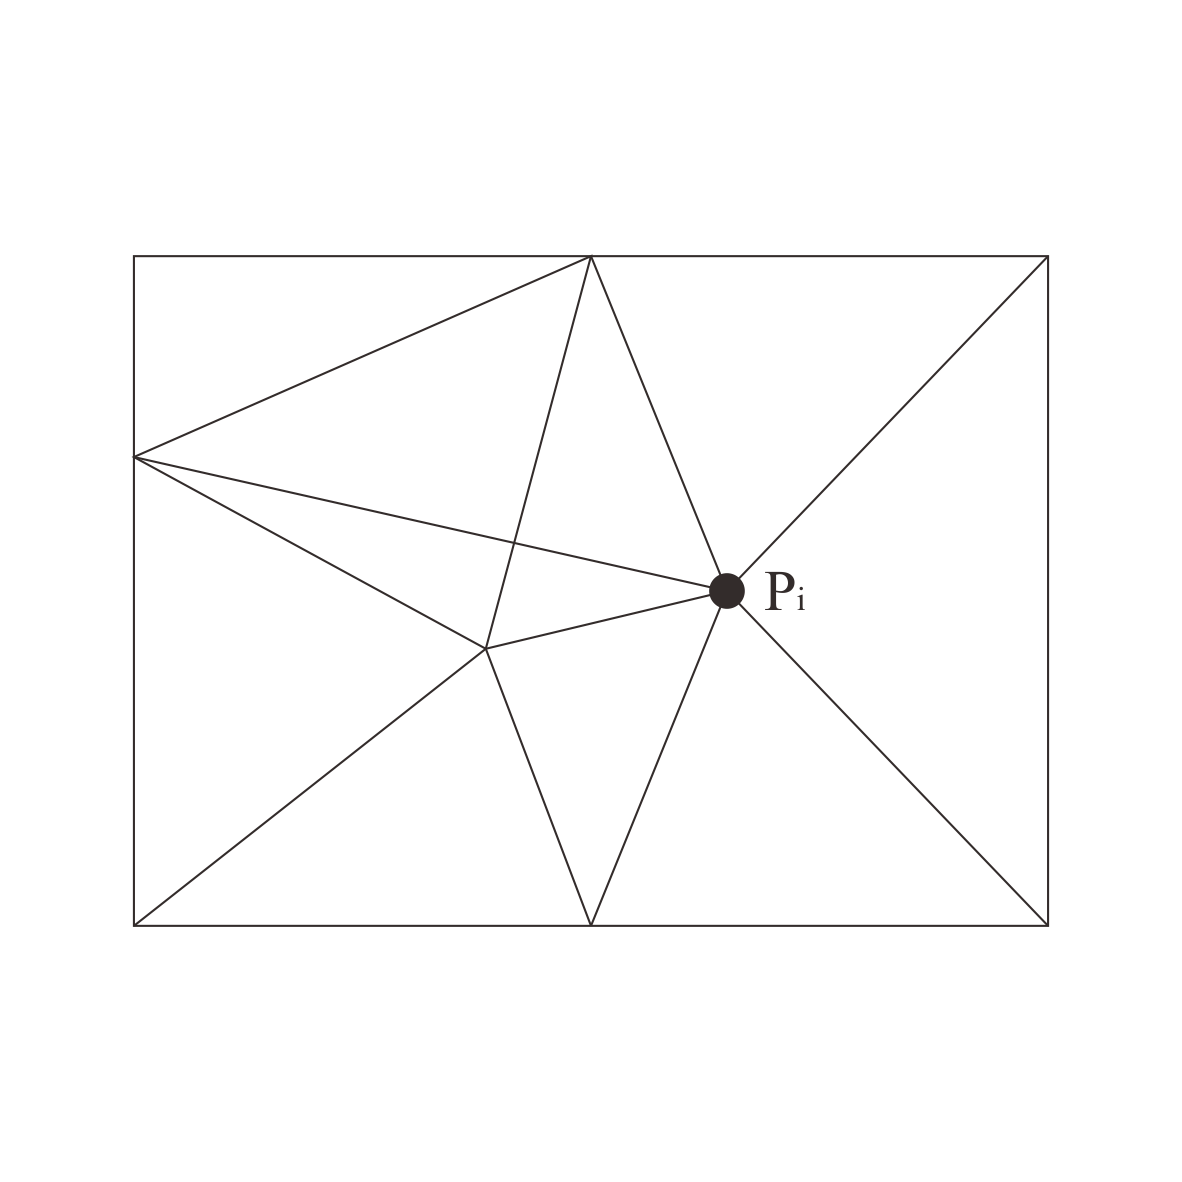
\includegraphics[width=0.55\linewidth]{picture/implement}
	\caption{}
	\label{fig:implement}
\end{figure}


For $ x = (x_1,x_2) \in \mathbb{R}^2 \text{ and } \forall v_h \in X_h $, we will have
\begin{eqnarray} \nonumber
v_h (\cdot) = \sum_{i=1}^{Np} v_h(P_i) \varphi_i(\cdot) &\in& X_h\\ \nonumber
w_h := \sum_{i=1}^{Np} v_h(P_i) \varphi_i &\in& X_h
\end{eqnarray}
such that
\begin{eqnarray}
 \nonumber
w_h(P_j) &=& \sum_{i=1}^{Np} v_h (P_i) \varphi_i (P_j)\\ \nonumber
&=& \sum_{i=1}^{Np} v_h (P_i) \delta_{ij}\\ \nonumber
&=& v_h (P_j)
\end{eqnarray}

Now, we consider basis of $ V_h $ for
\begin{eqnarray} \nonumber
\Omega \cap \Gamma &=& \emptyset \\ \nonumber
\{\varphi_i ; P_i \in \Omega \} &\subset& \{P_i \}_{i=1}^{Np}.
\end{eqnarray}
For simplicity, we assume $ \{\varphi_i ; P_i \in \Omega \} = \{P_i\}_{i=1}^N $ for $(N < Np) $, such that $ \{P_i\}_{i=1}^N \subset \Omega $ and $ \{P_i\}_{i=N+1}^{Np} \subset \Gamma $. 

Let $ V_h = \langle \varphi_1, \cdots , \varphi_N \rangle $, then 
\begin{equation*}
a(u_h , v_h)=l(v_h), \ (\forall v_h \in V_h) \ \Leftrightarrow \ a(u_h , \varphi_i) = l(\varphi_i), \ (i=1, \cdots , N).
\end{equation*}
If we choose $ v_h = \varphi_i \in V $, then $ \forall v_h \in V_h $ with $ c_i = v_h (P_i) $ and $ v_h = \sum_{i=1}^{N} c_i \varphi_i $,
\begin{eqnarray}\nonumber
a(u_h,v_h) &=& a(u_h,\sum_{i=1}^{N} c_i \varphi_i)\\ \nonumber
&=&\sum_{i=1}^{N} c_i a (u_h, \varphi_i) \\ \nonumber
&=& \sum_{i=1}^{N} c_i l(\varphi_i)\\ \nonumber
&=& l(\sum_{i=1}^{N} c_i \varphi_i) \\ \nonumber
&=& l(v_h)
\end{eqnarray}

We set $ u_j := u_h(P_j)$ for $ j=1, \cdots , Np $ such that at the boundary $ P_j \in \Gamma $ or for $ j=N+1, \cdots, Np $
\begin{equation*}
u_j = g_j = g_h(P_j), \ u_h \in V_h(g_h)
\end{equation*}
with $ u_{1}, \cdots, u_{N} $ is unknown.

Then, we can conclude that
\begin{equation*} 
\begin{cases}
a(u_h, \varphi_i) = l(\varphi_i), \ (i=1, \cdots , N)\\
u_h = \sum_{j=1}^{N} \ u_j \varphi_j + \sum_{j=N+1}^{Np} \ g_j \varphi_j, \ (u_h \in V_h (g_h))
\end{cases}.
\end{equation*}
For simplicity, we set notation $ a_{ij} := a(\varphi_i, \varphi_j) = a(\varphi_j, \varphi_i)$ such that for $  i=1, \cdots , N $,
\[\sum_{j=1}^{N} a_{ij} u_{j} + \sum_{j=N+1}^{Np} a_{ij} g_j = l(\varphi_i)\]

As conclusion, 
\[ a(u_h , v_h)=l(v_h), \ (\forall v_h \in V_h) \Leftrightarrow \mathbf{A} \mathbf{u} = \mathbf{b} \]
where
\begin{eqnarray}\nonumber
A &:=& (a_{ij}) \in \mathbb{R}_{\text{sym}}^{N \times N}\\ \nonumber
\text{\textbf{u}} &:=& \begin{pmatrix}
u_i \\ \vdots \\ u_{N}
\end{pmatrix}\\ \nonumber
\text{\textbf{b}} &:=& \Big(l(u_i) - \sum_{j=N+1}^{Np} a_{ij} g_j\Big) \text{, for }{i=1, \cdots , N}
\end{eqnarray}

\subsubsection{GIT}

\subsection{25 Desember 2017}

\subsubsection{Calculate matrix $ \mathbf{A}$}
\begin{eqnarray}\nonumber
A_{ij} &=& a(\varphi_{j}, \varphi_{i}) \\ \nonumber
&=& \int_{\Omega} \nabla \varphi_{j}(x) \cdot \nabla \varphi_{i}(x) \ dx \\ \nonumber
&=& \sum_{k=1}^{Ne} \int_{K_{k}} \nabla \varphi_{j}(x) \cdot \nabla \varphi_{i}(x) \ dx \\ \nonumber
&=& \sum_{k=1}^{Ne} \int_{K_{k}} 1 \ dx \ \big( \nabla \varphi_{j}(x) \cdot \nabla \varphi_{i}(x)\big).
\end{eqnarray}
To calculate it, usually we need $ N^3 $ computation for code like \\
\textgreater \hspace{1cm} for $ i=1, \dots, Np \  \{$ \\
\textgreater \hspace{1.5cm} for $ j=1, \dots , Np  \ \{$\\
\textgreater \hspace{2cm} for $ k=1, \dots, Ne \ \{ $  \\
\textgreater \hspace{2.5cm} $ A_{ij} = A_{ij} + \int_{K_{k}} \nabla\varphi_{j}(x) \cdot \nabla \varphi_{i}(x) dx $\\
\textgreater \hspace{2cm} $ \} $ \\
\textgreater \hspace{1.5cm} $ \} $ \\
\textgreater \hspace{1cm} $ \} $

But, we can simplify it into $ N^2 $ computation using local matrix and global matrix as shown below.\\
\textgreater \hspace{1cm} for $ k=1, \dots, Ne \ \{$\\
\textgreater \hspace{1.5cm} (local matrix)\\
\textgreater \hspace{1.5cm} $ A_{11}^{k} = \int_{K_{k}} \nabla \varphi_{1}(x) \cdot \varphi_{1}(x) \ dx $ \\
\textgreater \hspace{1.5cm} $ A_{12}^{k} = \int_{K_{k}} \nabla \varphi_{2}(x) \cdot \varphi_{1}(x) \ dx $ \\
\textgreater \hspace{3.5cm} $ \vdots $ \\
\textgreater \hspace{1.5cm} $ A_{33}^{k} = \int_{K_{k}} \nabla \varphi_{3}(x) \cdot \varphi_{3}(x) \ dx $ \\
\textgreater \hspace{1.5cm} (global matrix) \\
\textgreater \hspace{1.5cm} $ A_{44}= A_{44} + A_{11}^{k}$ \\
\textgreater \hspace{1.5cm} $ A_{47}= A_{47} + A_{12}^{k}$ \\
\textgreater \hspace{2.5cm} $ \vdots $ \\
\textgreater \hspace{1.5cm} $ A_{73}= A_{73} + A_{23}^{k}$ \\
\textgreater \hspace{2.5cm} $ \vdots $ \\
\textgreater \hspace{1.5cm} $ A_{33}= A_{33} + A_{33}^{k}$ \\
\textgreater \hspace{1cm} $ \}$ \\

\subsubsection{Calculate vector $ \mathbf{B} $}
\begin{eqnarray} \nonumber
b_{i} &=& \int_{\Omega} f(x) \varphi_{i}(x) \ dx - \sum_{j=1}^{Np} g_{h}(P_{j}) \int_{\Omega} \nabla \varphi_{j}(x) \cdot \nabla \varphi_{i}(x) \ dx \\ \nonumber
&=& \sum_{k=1}^{Ne} \int_{K_{k}} f(x) \varphi_{i}(x) \ dx - \sum_{j=1}^{Np} g_{h}(P_{j}) \sum_{k=1}^{Ne} \int_{K_{k}} \nabla \varphi_{j}(x) \cdot \nabla \varphi_{i}(x) \ dx
\end{eqnarray}
Consider $ g_{h}(P_{j}) = 0 $, with $ f_{h}(x) = \sum_{j=1}^{Np} f(P_{j})\varphi_{j}(x) $ then for each element,
\begin{eqnarray} \nonumber
b_{i} &=& b_{i} + \int_{K_{k}} f(x) \varphi_{i}(x) \ dx \\ \nonumber
&=& b_{i} + \int_{K_{k}} \Big( f(P_{1}) \varphi_{1}(x) + f(P_{2}) \varphi_{2}(x) + f(P_{3}) \varphi_{3}(x) \Big) \varphi_{i}(x) \ dx \\ \nonumber
&=& b_{i} + \int_{K_{k}} f(P_{1}) \varphi_{1}(x) \cdot \varphi_{i}(x) + f(P_{2}) \varphi_{2}(x) \cdot \varphi_{i}(x) + f(P_{3}) \varphi_{3}(x) \cdot \varphi_{i}(x) \ dx \\ \nonumber
&=& b_{i} + f(P_{1}) \int_{K_{k}} \varphi_{1}(x) \cdot \varphi_{i}(x) \ dx + f(P_{2}) \int_{K_{k}} \varphi_{2}(x) \cdot \varphi_{i}(x) \ dx + \\ \nonumber
& & f(P_{3}) \int_{K_{k}} \varphi_{3}(x) \cdot \varphi_{i}(x) \ dx
\end{eqnarray}
with
\[  \int_{K_{k}} \varphi_{i}(x) \varphi_{j}(x) = \begin{cases}
\dfrac{meas(K_{k})}{6}, & for \ i=j \\
\dfrac{meas(K_{k})}{12}, & for \ i \neq j 
\end{cases} \]


(way to calculate in program)

\subsubsection{Other calculation}
For any points $ P_{i}(x_{1},x_{2}) $ in triangle $ K $,
\begin{figure}
	\centering
	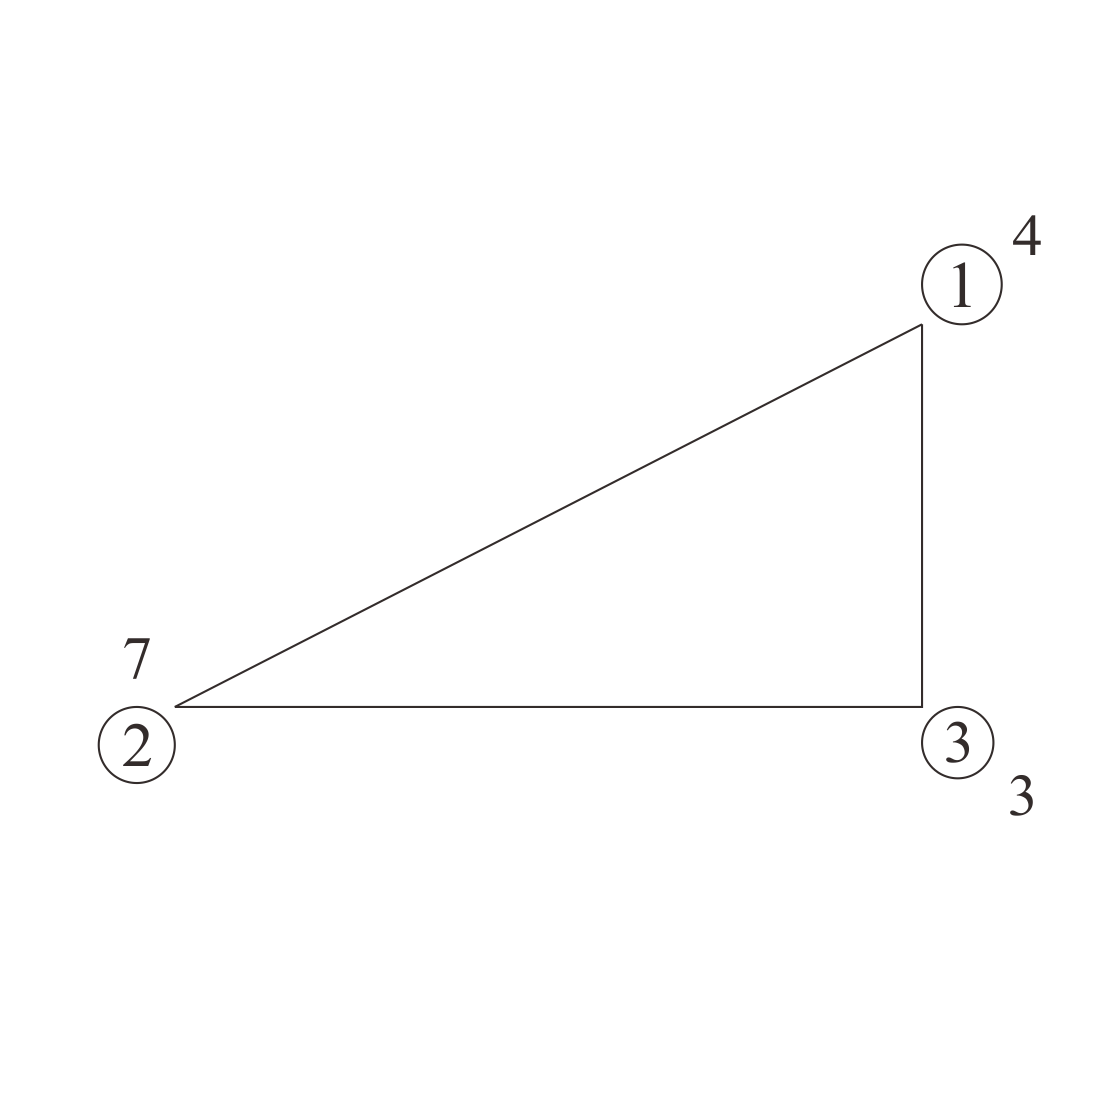
\includegraphics[width=0.6\linewidth]{picture/triangle}
	\caption{}
	\label{fig:triangle}
\end{figure}

\[ \varphi_{i}(x) = c_{0} + c_{1}x_{1} +  c_{2}x_{2}, \ c_{j} \in \mathbb{R} \]
such that
\[ \nabla \varphi_{i}(x) = \begin{pmatrix}
c_{1} \\ c_{2}
\end{pmatrix}.  \]
To compute the triangle area $ \int_{K_{k}} 1 \ dx $,


\subsection{5 January 2018 (Error Estimate)}
\subsubsection{Norm}
After find the solution $ u(x) $, we should check if the solution we found is close enough to the exact solution. For numerical solution $ u_{h} $, we check for $ h = \dfrac{1}{N} $ where $ N $  or devider of each boundary side is set to $ N = 4,8,16,32 $.

In this problem we set $ f(x) = -\nabla u(x) = 2 \pi^2(sin(x\pi)sin(y\pi))$ with exact solution $ u_{e}(x) = sin(x\pi)sin(y\pi) $. We want to calculate $ \Vert u_{h}-\Pi_{h}u_{e} \Vert_{X} ,s \ X = L^2(\Omega), H_{0}^{1}(\Omega)$. Here, $ \Pi_{h} $ is function that mapping continuous function $ C(\bar{\Omega}) $ into piecewise linear finite element space.
\begin{eqnarray}\nonumber
\Pi_{h} : & C(\bar{\Omega}) & \rightarrow P1-FEsp \\ \nonumber
& v & \mapsto \Pi_{h}v
\end{eqnarray}
such that $ (\Pi_{h}v)(P) := v(P) $, $ P $ is nodes.

\begin{figure}[h!]
	\centering
	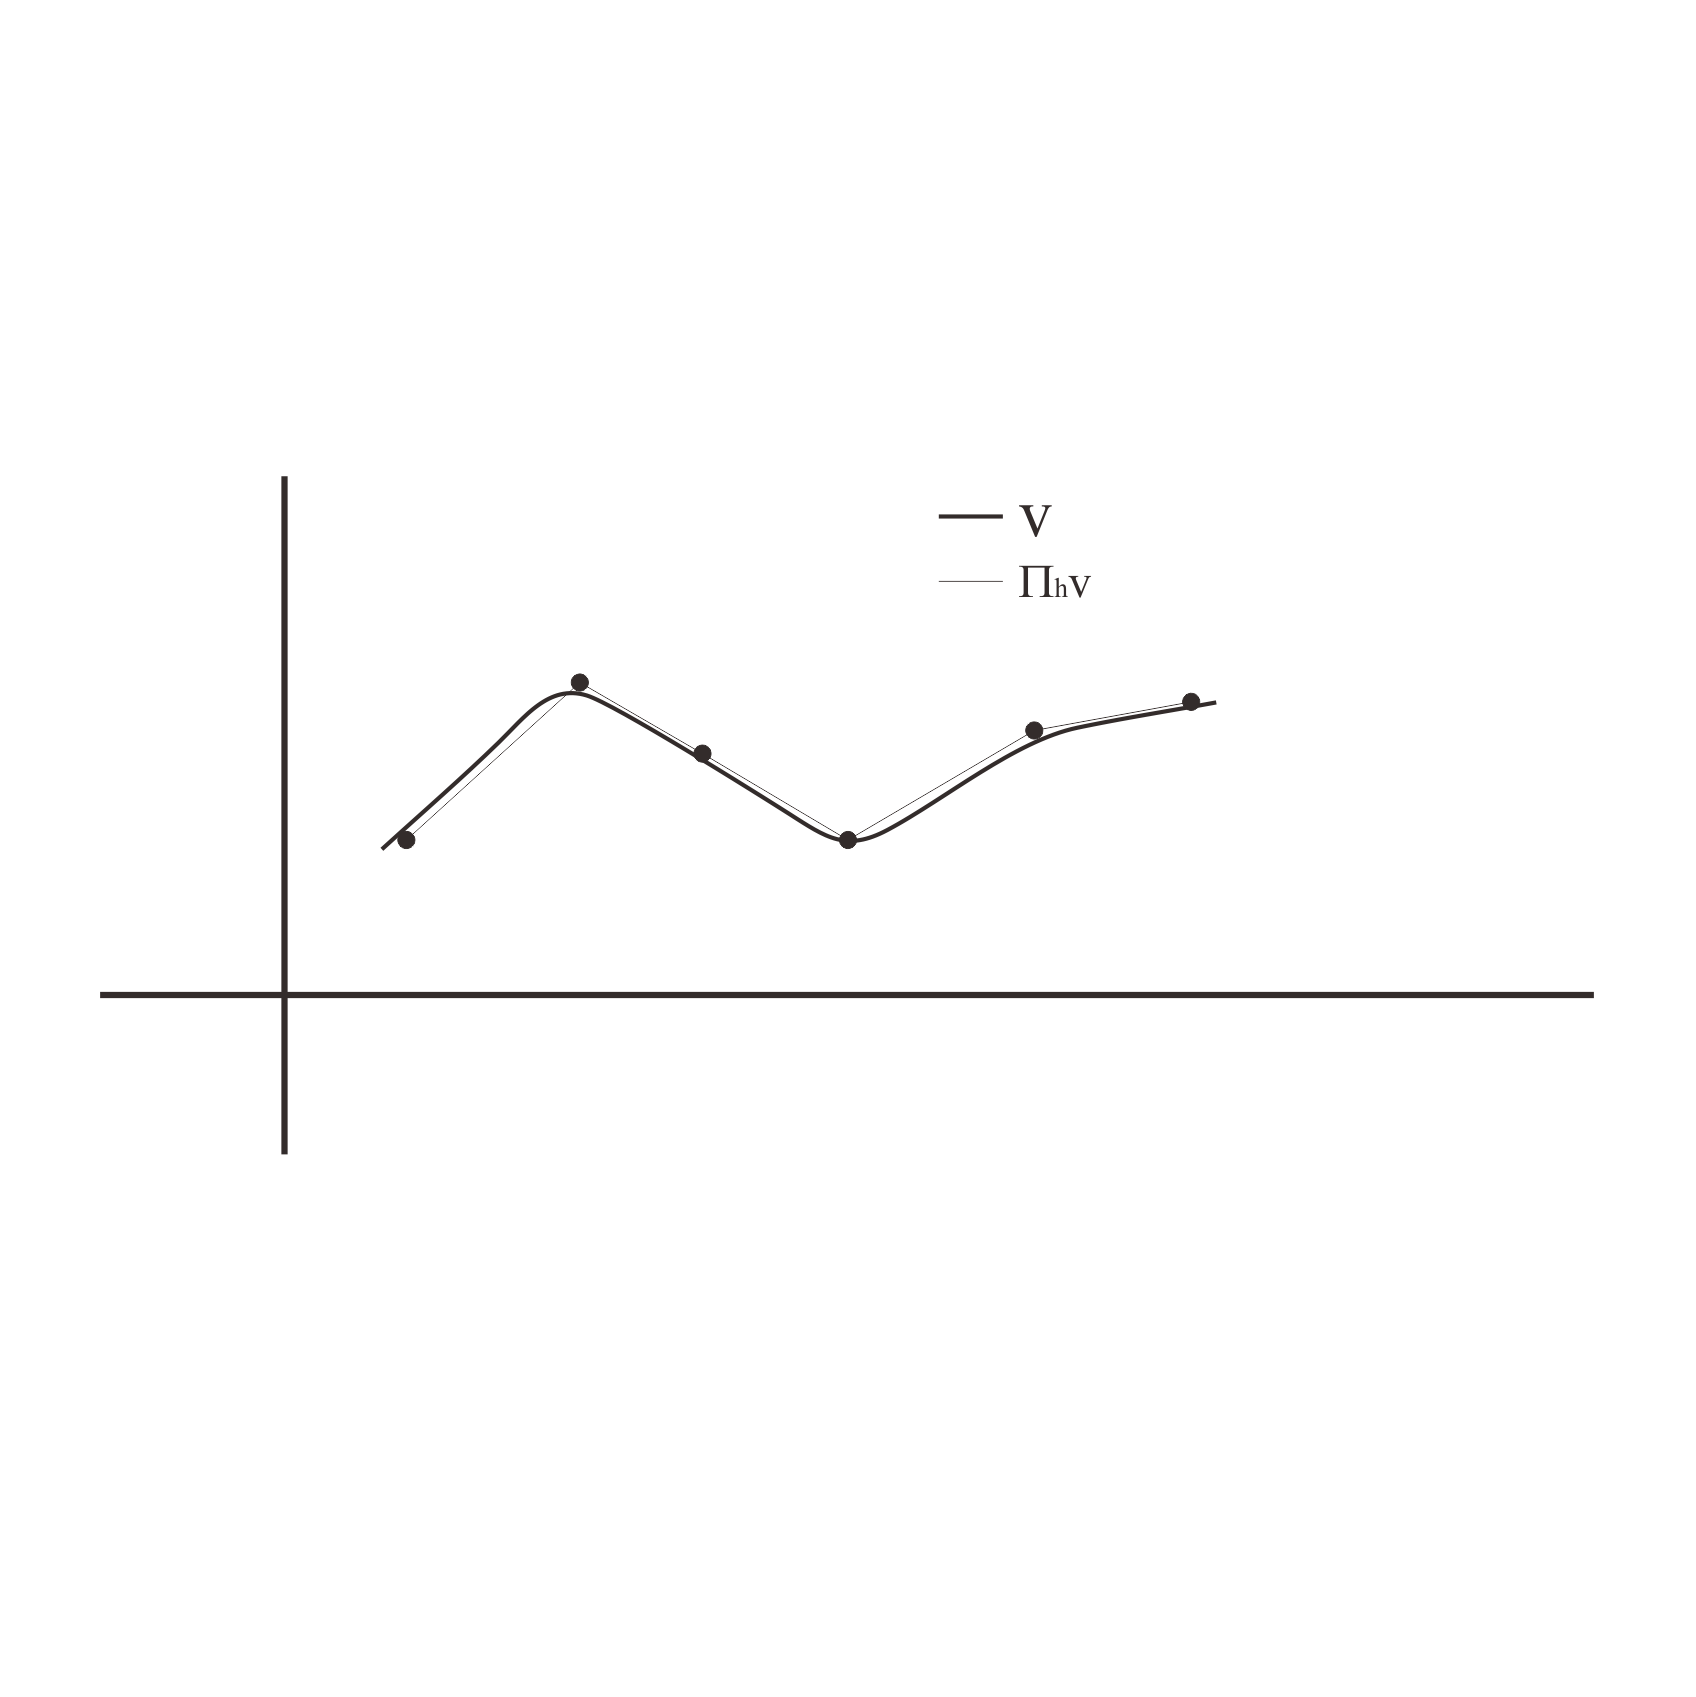
\includegraphics[width=0.7\linewidth]{picture/grafik1}
	\caption{}
	\label{fig:grafik1}
\end{figure}

\subsubsection{$ L^2(\Omega) $ norm}
\begin{eqnarray}\nonumber
\Vert v_{h} \Vert_{L^2(\Omega)} &=& \sqrt{\int_{\Omega} \big(v_{h}(x)\big)^2 \ dx} \\ \nonumber
&=& \sqrt{ \sum_{K} \int_{K} \big(v_{h}(x)\big)^2 \ dx} \\ \nonumber
&=& \sqrt{ \sum_{K} \int_{K} \big( v_{i}\varphi_{i}^{(K)}(x) + v_{j}\varphi_{j}^{(K)}(x) + v_{k}\varphi_{k}^{(K)}(x) \big)^2 \ dx} \\ \nonumber
&=& \sqrt{ \sum_{K} \int_{K} \Big(
	\begin{pmatrix}
	v_{i} & v_{j} & v_{k}
	\end{pmatrix}
	\begin{pmatrix}
	\varphi_{i}^{(K)}(x) \\ \varphi_{j}^{(K)}(x) \\ \varphi_{k}^{(K)}(x) 
	\end{pmatrix}
	\Big)^2 \ dx} \\\ \nonumber
&=& \sqrt{ \sum_{K} \int_{K}
	\begin{pmatrix}
	v_{i} & v_{j} & v_{k}
	\end{pmatrix}
	\begin{pmatrix}
	\varphi_{i}^{(K)}(x) \\ \varphi_{j}^{(K)}(x) \\ \varphi_{k}^{(K)}(x) 
	\end{pmatrix}
	\begin{pmatrix}
	\varphi_{i}^{(K)}(x) & \varphi_{j}^{(K)}(x) & \varphi_{k}^{(K)}(x) 
	\end{pmatrix}
	\begin{pmatrix}
	v_{i} \\ v_{j} \\ v_{k}
	\end{pmatrix} \ dx} \\ \nonumber
&=& \sqrt{ \sum_{K}
	\begin{pmatrix}
	v_{i} & v_{j} & v_{k}
	\end{pmatrix}
	\int_{K}
	\begin{pmatrix}
	\varphi_{i}^{(K)}\cdot\varphi_{i}^{(K)} & \varphi_{i}^{(K)}\cdot\varphi_{j}^{(K)} & \varphi_{i}^{(K)}\cdot\varphi_{k}^{(K)} \\ \varphi_{j}^{(K)}\cdot\varphi_{i}^{(K)} & \varphi_{j}^{(K)}\cdot\varphi_{j}^{(K)} & \varphi_{j}^{(K)}\cdot\varphi_{k}^{(K)}  \\ \varphi_{k}^{(K)}\cdot\varphi_{i}^{(K)} & \varphi_{k}^{(K)}\cdot\varphi_{j}^{(K)} & \varphi_{k}^{(K)}\cdot\varphi_{k}^{(K)} 
	\end{pmatrix}
	\ dx
	\begin{pmatrix}
	v_{i} \\ v_{j} \\ v_{k}
	\end{pmatrix}} \\ \nonumber
&=& \sqrt{ \sum_{K}
	\begin{pmatrix}
	v_{i} & v_{j} & v_{k}
	\end{pmatrix}
	\dfrac{\vert K \vert}{12}
	\begin{pmatrix}
	2 & 1 & 1 \\ 1 & 2 & 1 \\ 1 & 1 & 2
	\end{pmatrix}
	\begin{pmatrix}
	v_{i} \\ v_{j} \\ v_{k}
	\end{pmatrix}} \\ \nonumber
&=& \sqrt{ \sum_{K}
	\dfrac{\vert K \vert}{12}
	\begin{pmatrix}
	2 & 1 & 1 \\ 1 & 2 & 1 \\ 1 & 1 & 2
	\end{pmatrix}
	v^{T} \cdot M \cdot v
	}
\end{eqnarray}
with
\[ v = \begin{pmatrix}
v_{i} \\ v_{j} \\ v_{k}
\end{pmatrix} \hspace{2cm}
M = \begin{pmatrix}
2 & 1 & 1 \\ 1 & 2 & 1 \\ 1 & 1 & 2
\end{pmatrix}  \]

In our problem, we need to find $ \Vert v_{h} \Vert_{L^2(\Omega)} = \Vert u_{h} - \Pi_{h}u_{e} \Vert_{L^2(\Omega)} $. Then we subtitute
\[ v_{h}(P) = u_{h}(P) - u_{e}(P) \]
for every point $ P $.

\begin{figure}[h!]
	\centering
	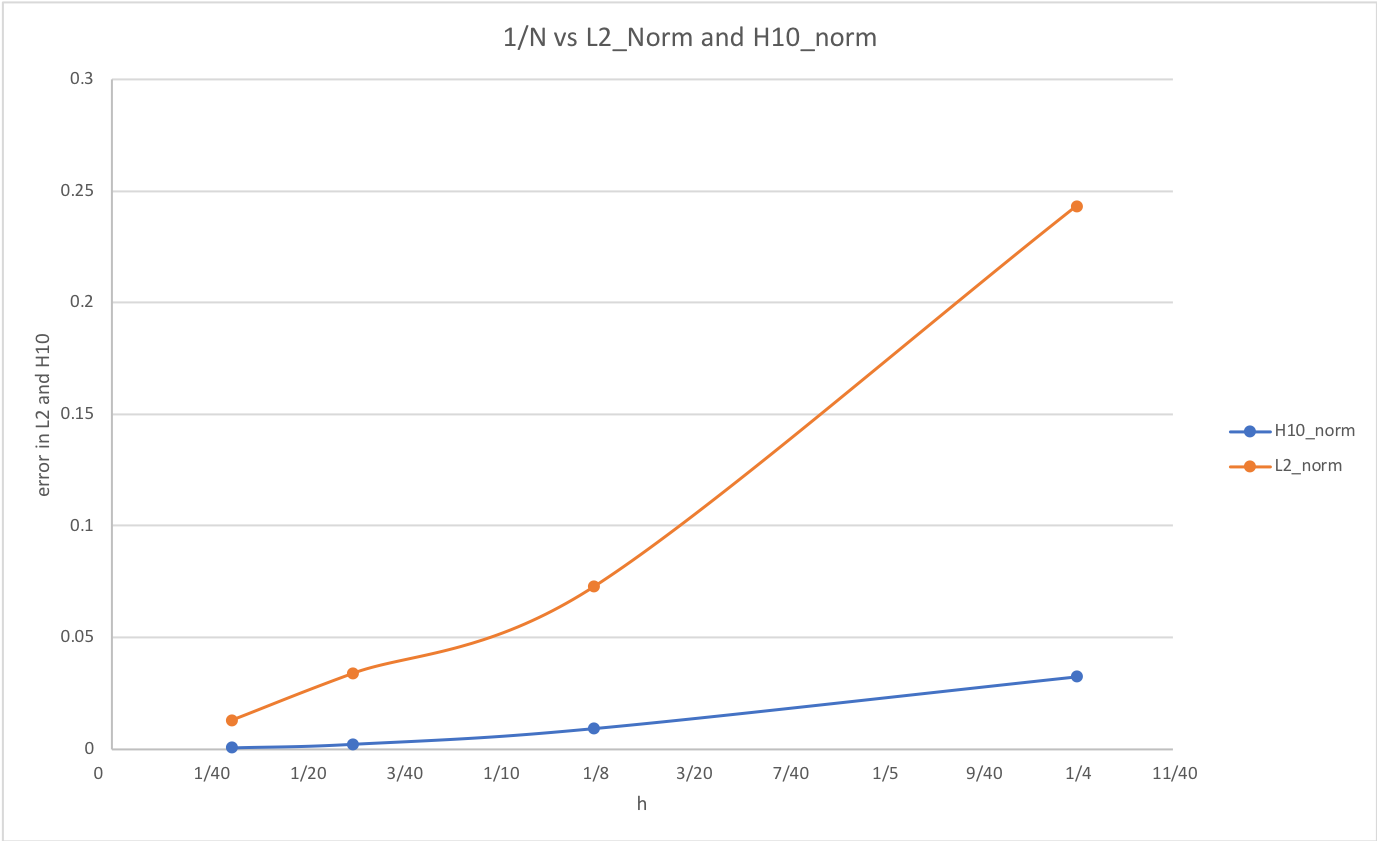
\includegraphics[width=0.7\linewidth]{picture/grafik2}
	\caption{}
	\label{fig:grafik2}
\end{figure}


\subsubsection{$ H_{0}^{1}(\Omega) $ norm}
\begin{eqnarray} \nonumber
\Vert v_{h} \Vert_{H_1^0(\Omega)} &=& \sqrt{\int_{\Omega} \nabla v_{h}(x) \cdot \nabla v_{h}(x) \ dx} \\ \nonumber
&=& \sqrt{\int_{\Omega} \vert \nabla v_{h}(x) \vert^{2} \ dx} \\ \nonumber
&=& \sqrt{\sum_{K} \vert \nabla v_{h}|_{K} (x) \vert^{2} \vert K \vert}
\end{eqnarray}
with $ \nabla v_{h}|_{K}(x) $ does not depend on $ x $
\[ \nabla v_{h}|_{K}(x) = v_{i} \begin{pmatrix} c_{1}^{(i)}\\ c_{2}^{(i)} \end{pmatrix} + v_{j} \begin{pmatrix} c_{1}^{(j)}\\ c_{2}^{(j)} \end{pmatrix} + v_{k} \begin{pmatrix} c_{1}^{(i)}\\ c_{2}^{(i)} \end{pmatrix}\] 

\end{document}